In the final section of this thesis, we will explore the fANOVA decomposition visually. This will provide better understanding for how fANOVA components behave in different scenarios; also if fANOVA should enhance interpretability, it is important to have visualizations of it. We will first revisit our running example and then explore some other functions.
\subsection{Comparison of Decompositions}
Recall our running example:
$$h(x_1, x_2) = x_1 + 2 x_2 + x_1 x_2,$$
with polynomial coefficients: $a_0 = 0$, $a_1 = 1$, $a_2 = 2$, $a_{11} = 0$, $a_{22} = 0$, $a_{12} = 1$.
Under independent inputs ($\rho = 0$), the fANOVA components are given by:
\begin{align*}
y_{\emptyset} &= 0, \\
y_1(x_1) &= x_1\\
y_2(x_2) &= 2x_2\\
y_{12}(x_1, x_2) &= x_1x_2,
\end{align*}
visualized in \autoref{fig:running_ex_independent}. As expected, we observe simple linear functions and a regular symmetric contour plot.
% Input: MVN, centred, independent
\begin{figure}[htpb]
    \centering
    \begin{subfigure}[t]{0.49\textwidth}
        \centering
        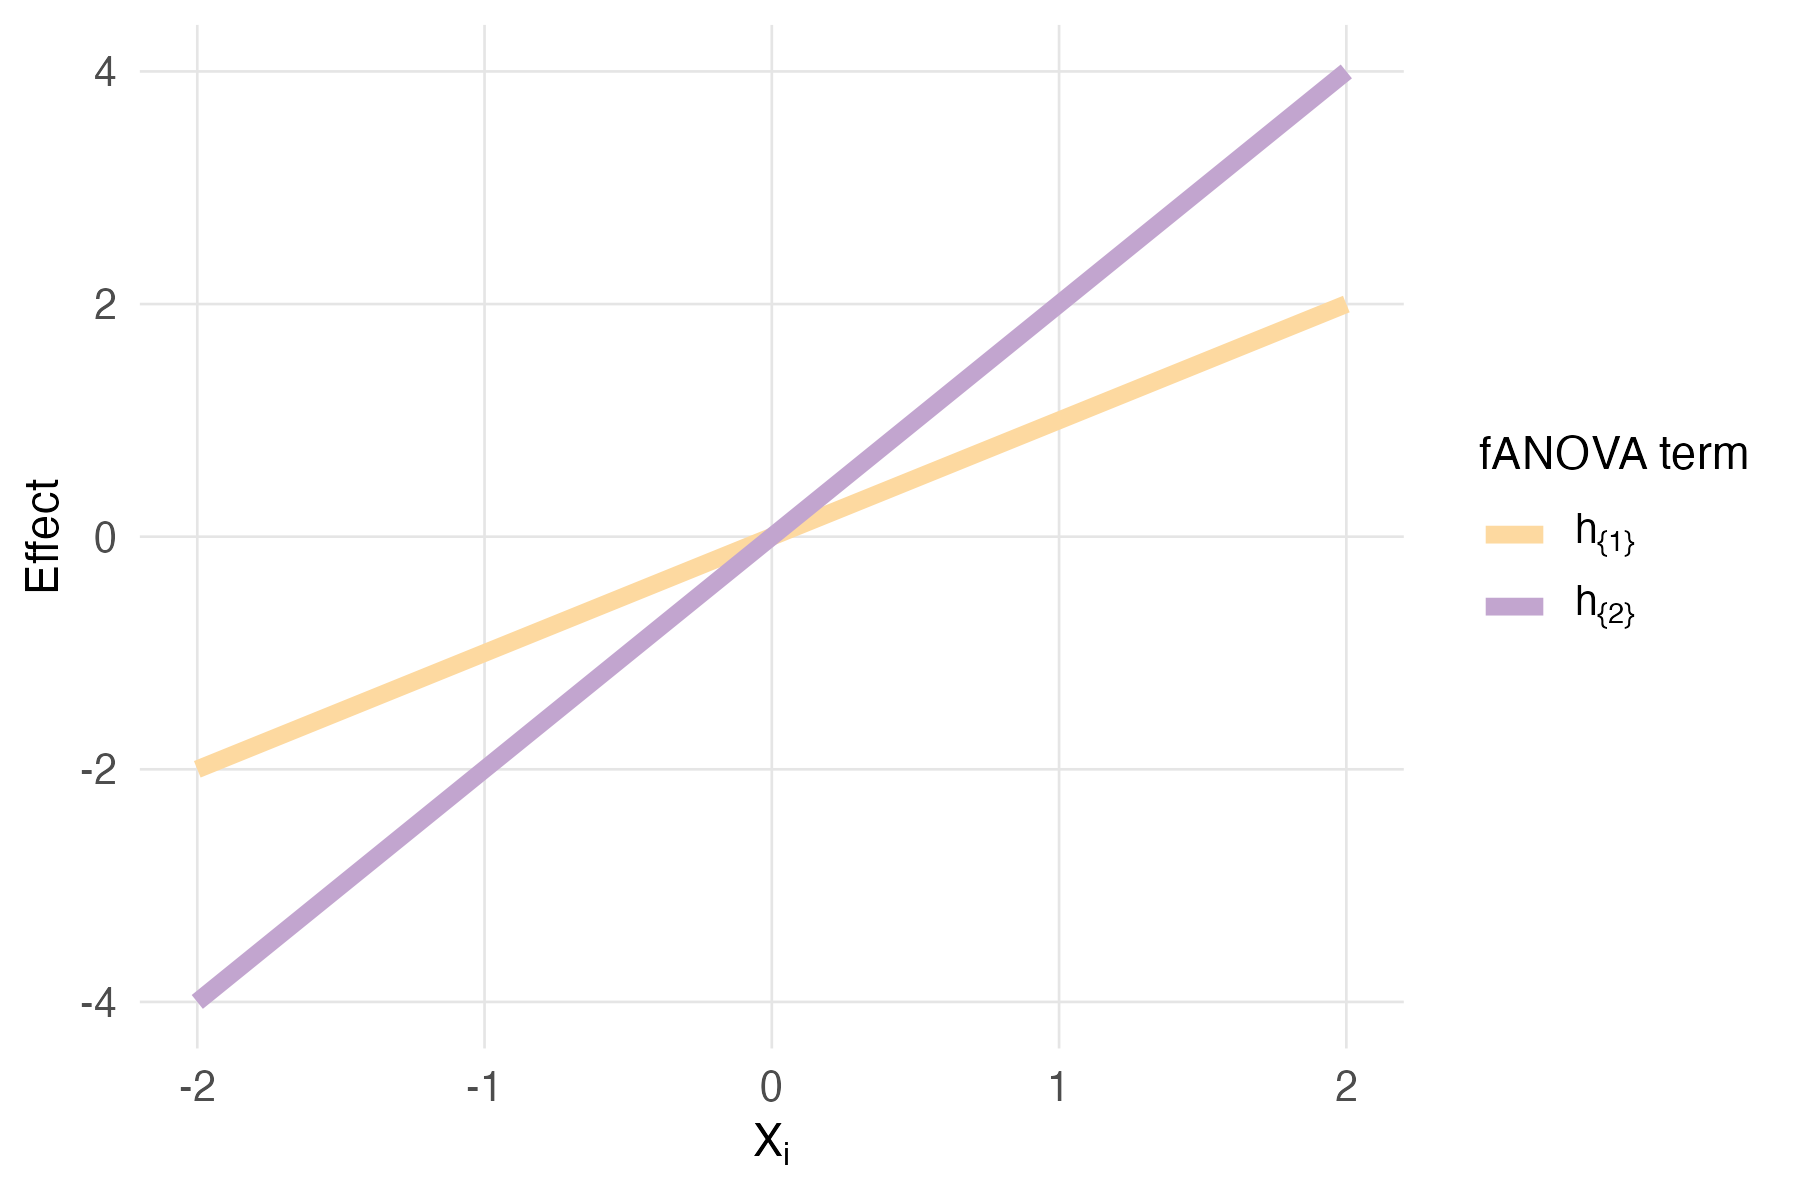
\includegraphics[width=\textwidth]{images/experiment_section/running_example_a1p10_a2p20_a11p00_a22p00_a12p10_rhop00_main.png}
    \end{subfigure}%
    \hfill
    \begin{subfigure}[t]{0.49\textwidth}
        \centering
        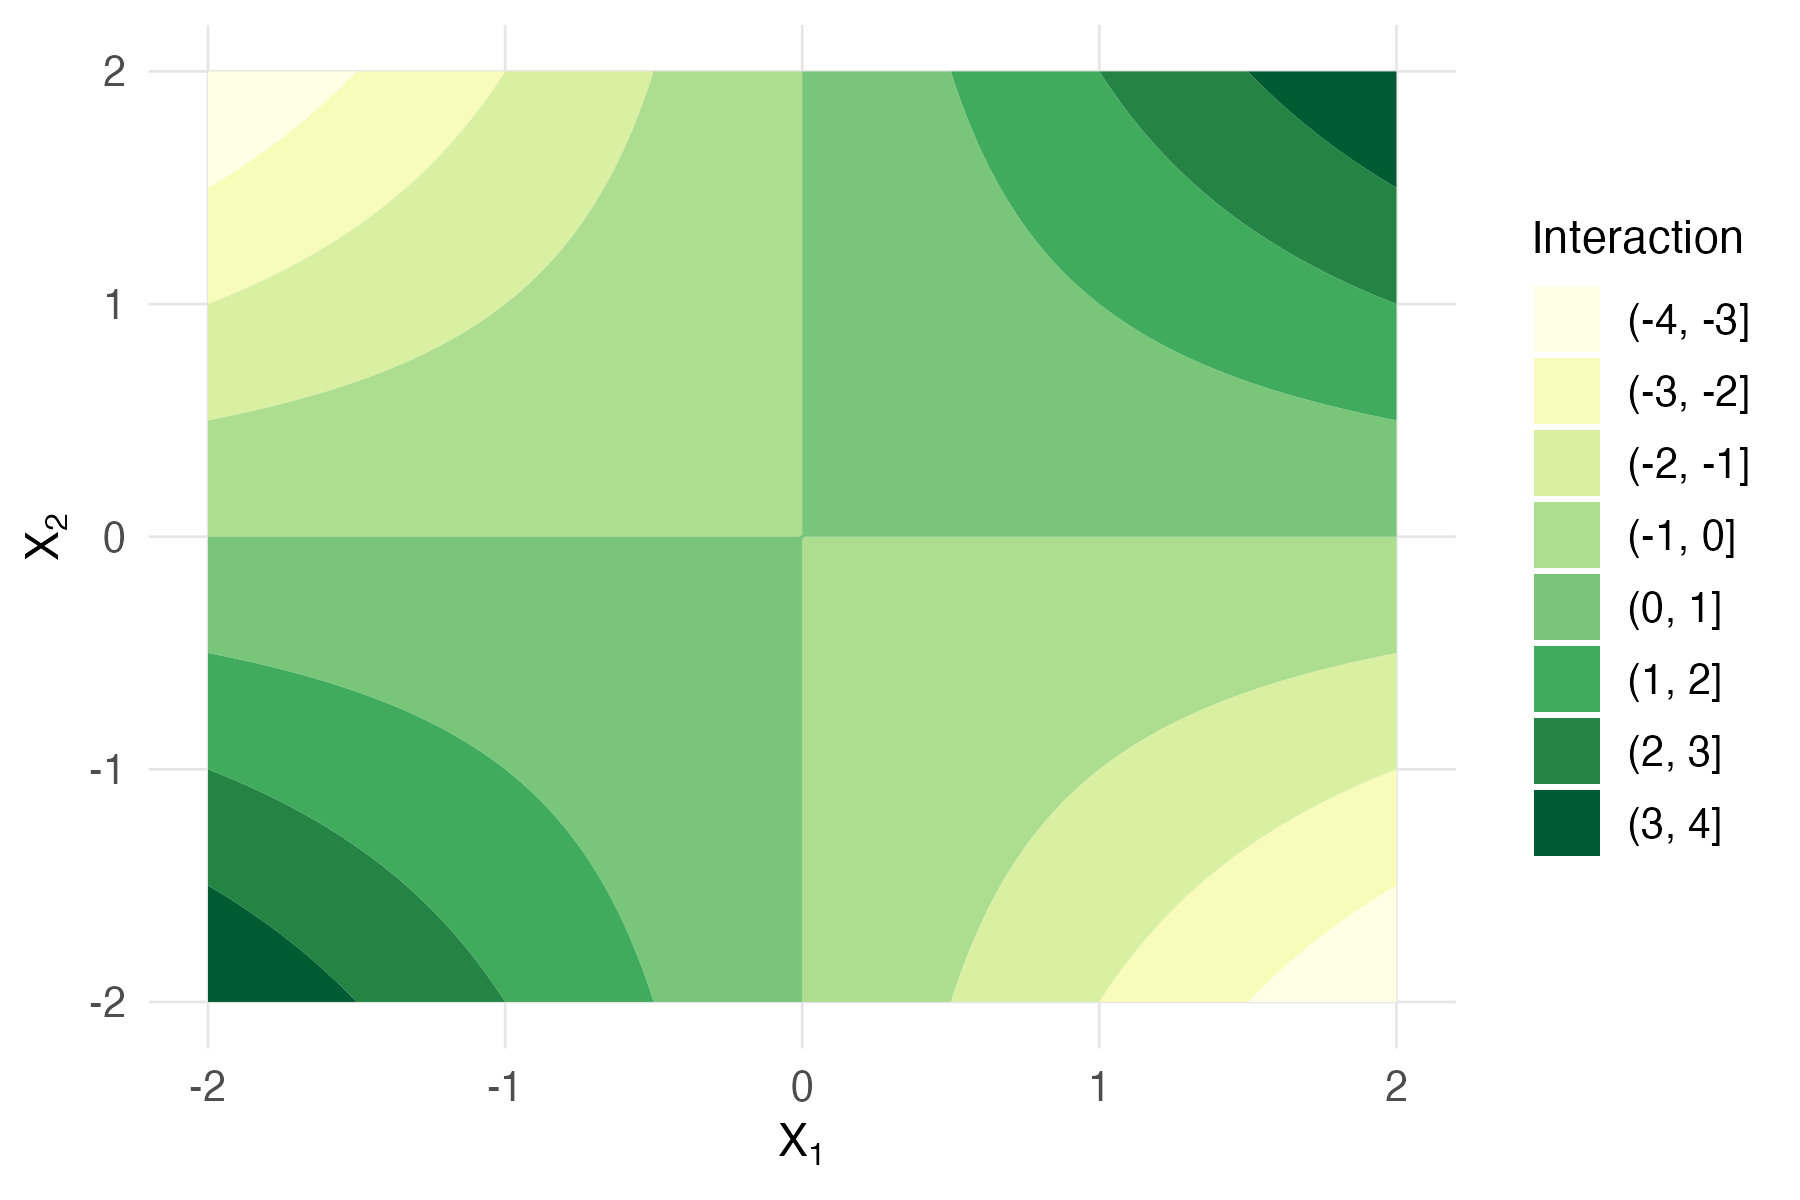
\includegraphics[width=\textwidth]{images/experiment_section/running_example_a1p10_a2p20_a11p00_a22p00_a12p10_rhop00_interaction.png}
    \end{subfigure}
    \caption{Main effects (left) and interaction effect (right) of the fANOVA decomposition for $h(x_1, x_2) = x_1 + 2 x_2 + x_1 x_2$ with independent inputs.}
    \label{fig:running_ex_independent}
\end{figure}

Now we assume $\rho = 0.5$. In attempt to compute the fANOVA terms under dependent inputs, we calculated the following effects, which do not satisfy the fANOVA property of orthogonality. Nevertheless, is it interesting to compare their visualization in \autoref{fig:hoeffding_rho05} to the one of the true generalized fANOVA components.
The main effects are parabolic, and the interaction term seems to be non-symmetric.

\begin{align*}
\tilde{y}_0 &= a + 0.5, \\[3pt]
\tilde{y}_1(x_1) &= 2x_1 + 0.5x_1^2 - 0.5, \\[3pt]
\tilde{y}_2(x_2) &= 2.5x_2 + 0.5x_2^2 - 0.5, \\[3pt]
\tilde{y}_{12}(x_1,x_2) &= x_1x_2 - x_1 - 0.5x_2 - 0.5x_1^2 - 0.5x_2^2 + 0.5,
\end{align*}

\begin{figure}[htpb]
    \centering
    \begin{subfigure}[t]{0.49\textwidth}
        \centering
        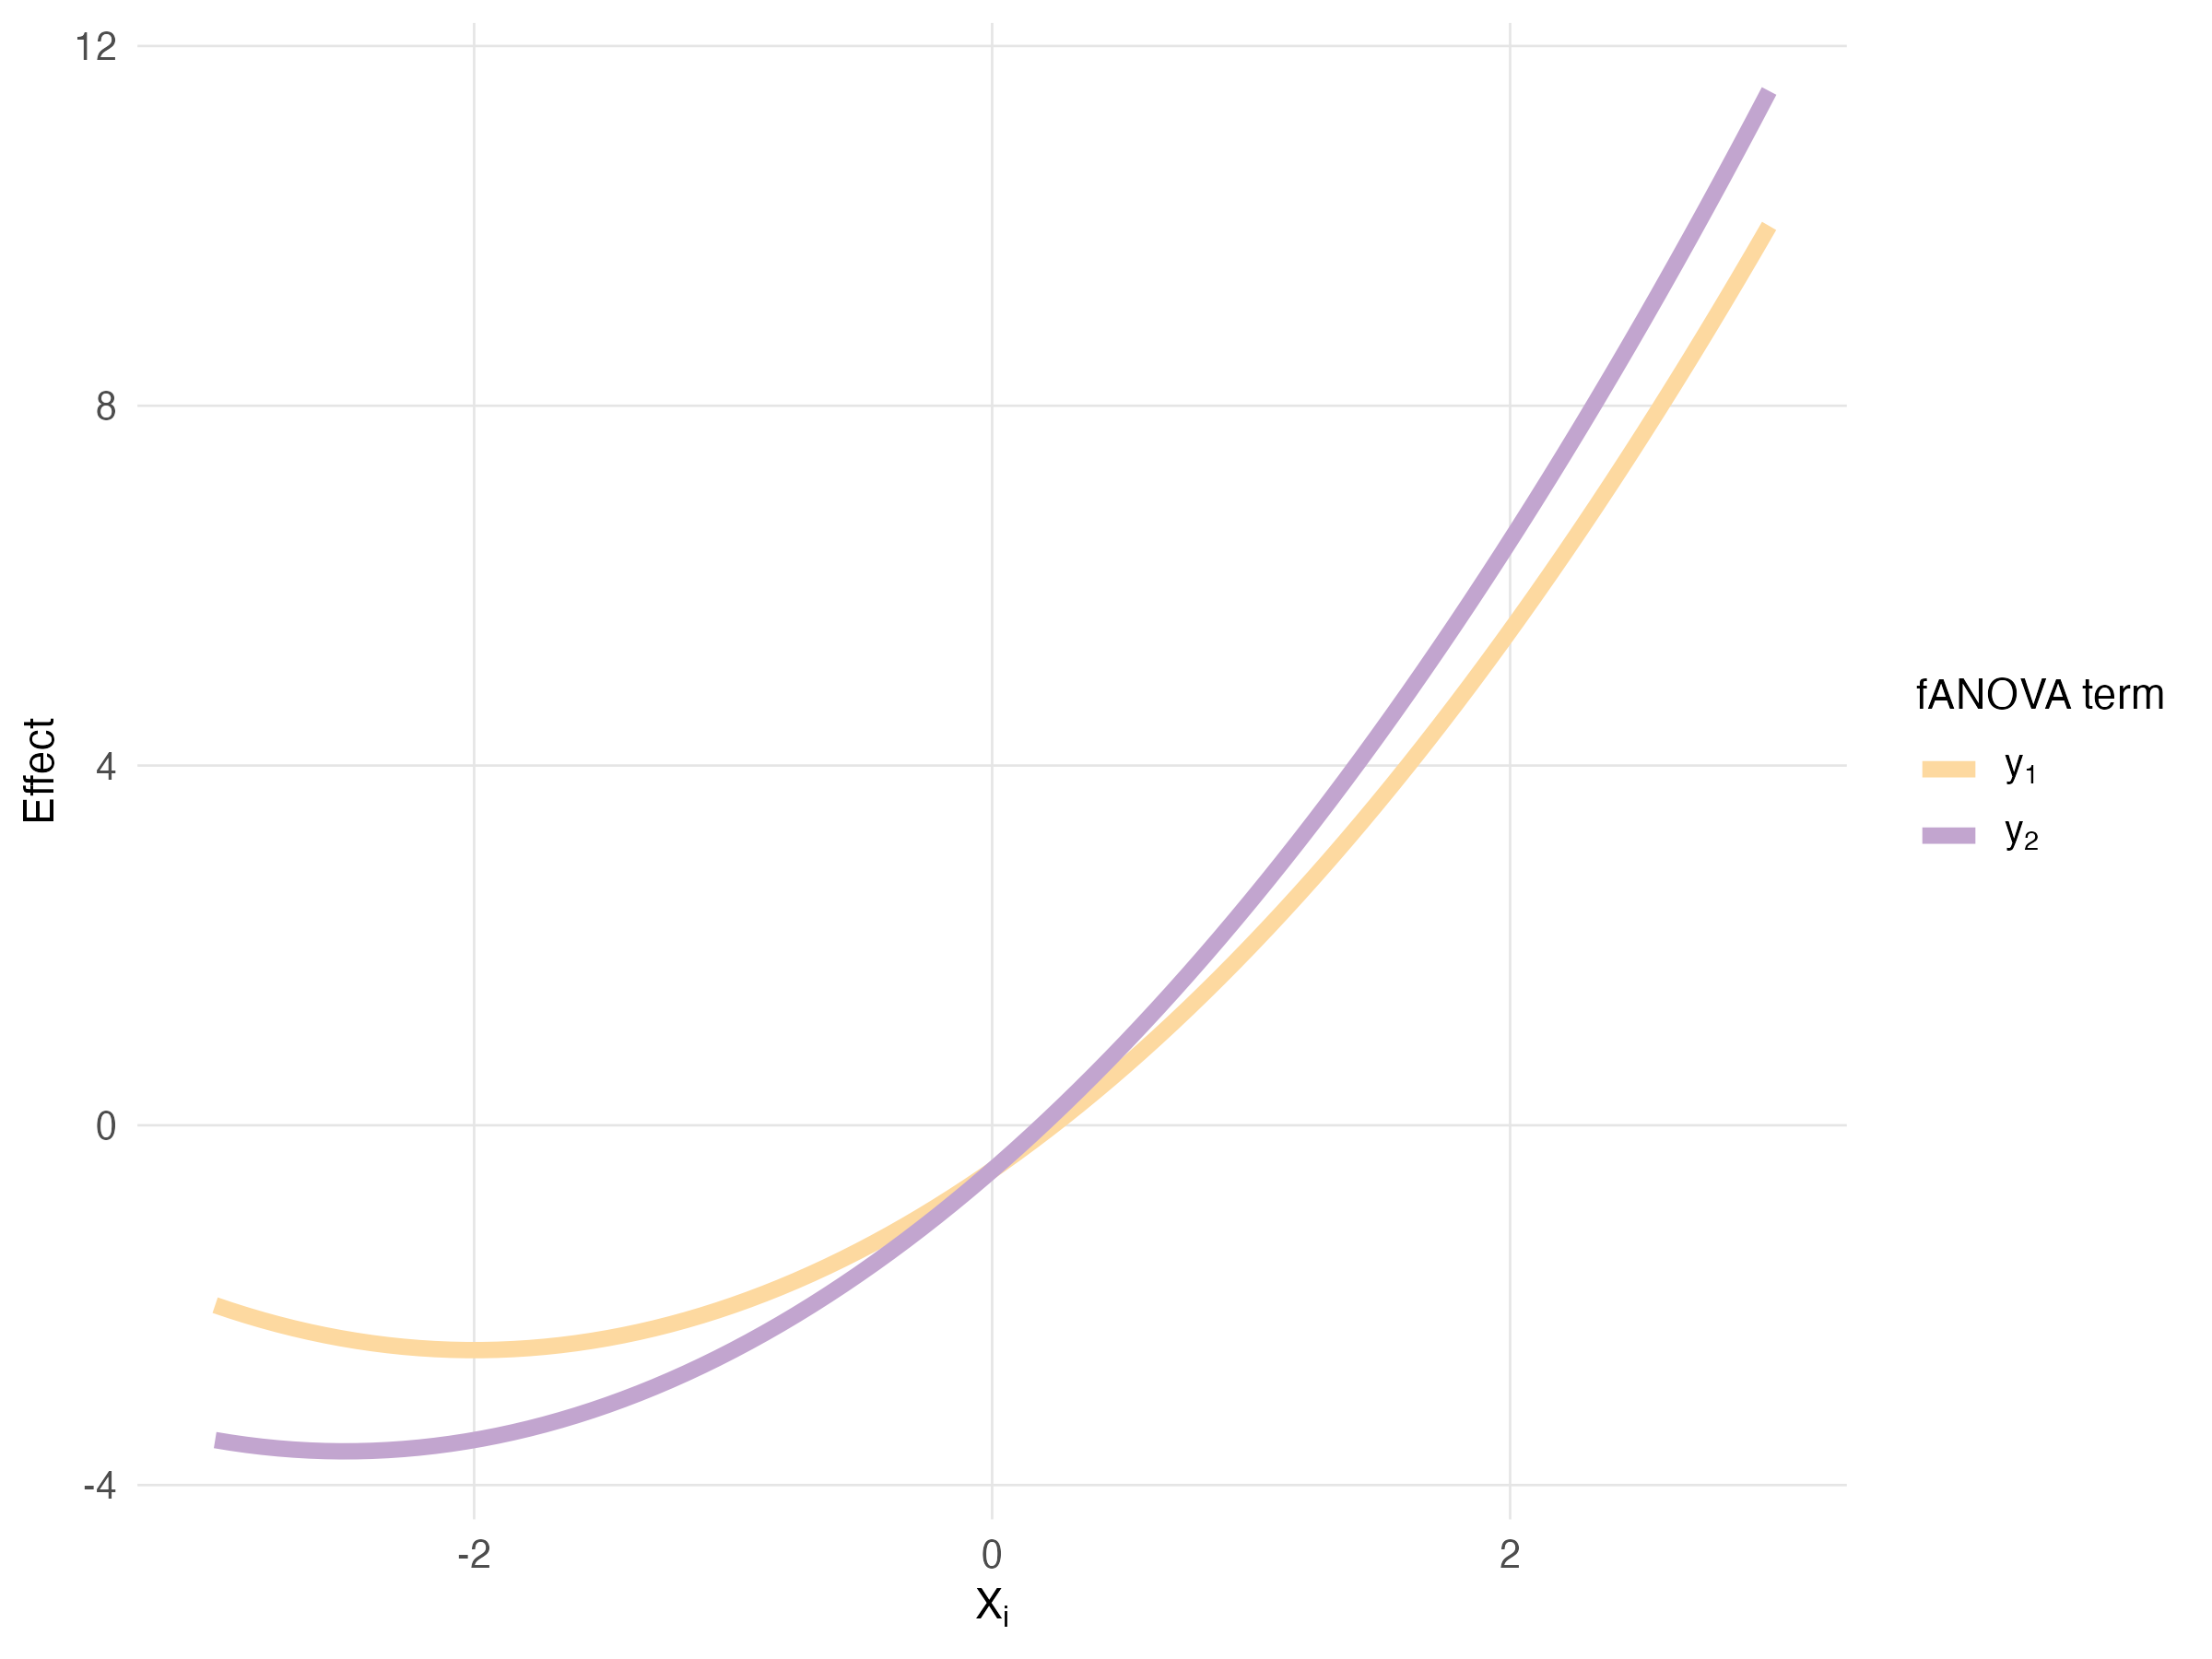
\includegraphics[width=\textwidth]{images/experiment_section/hoeffding_rho05_main.png}
    \end{subfigure}%
    \hfill
    \begin{subfigure}[t]{0.49\textwidth}
        \centering
        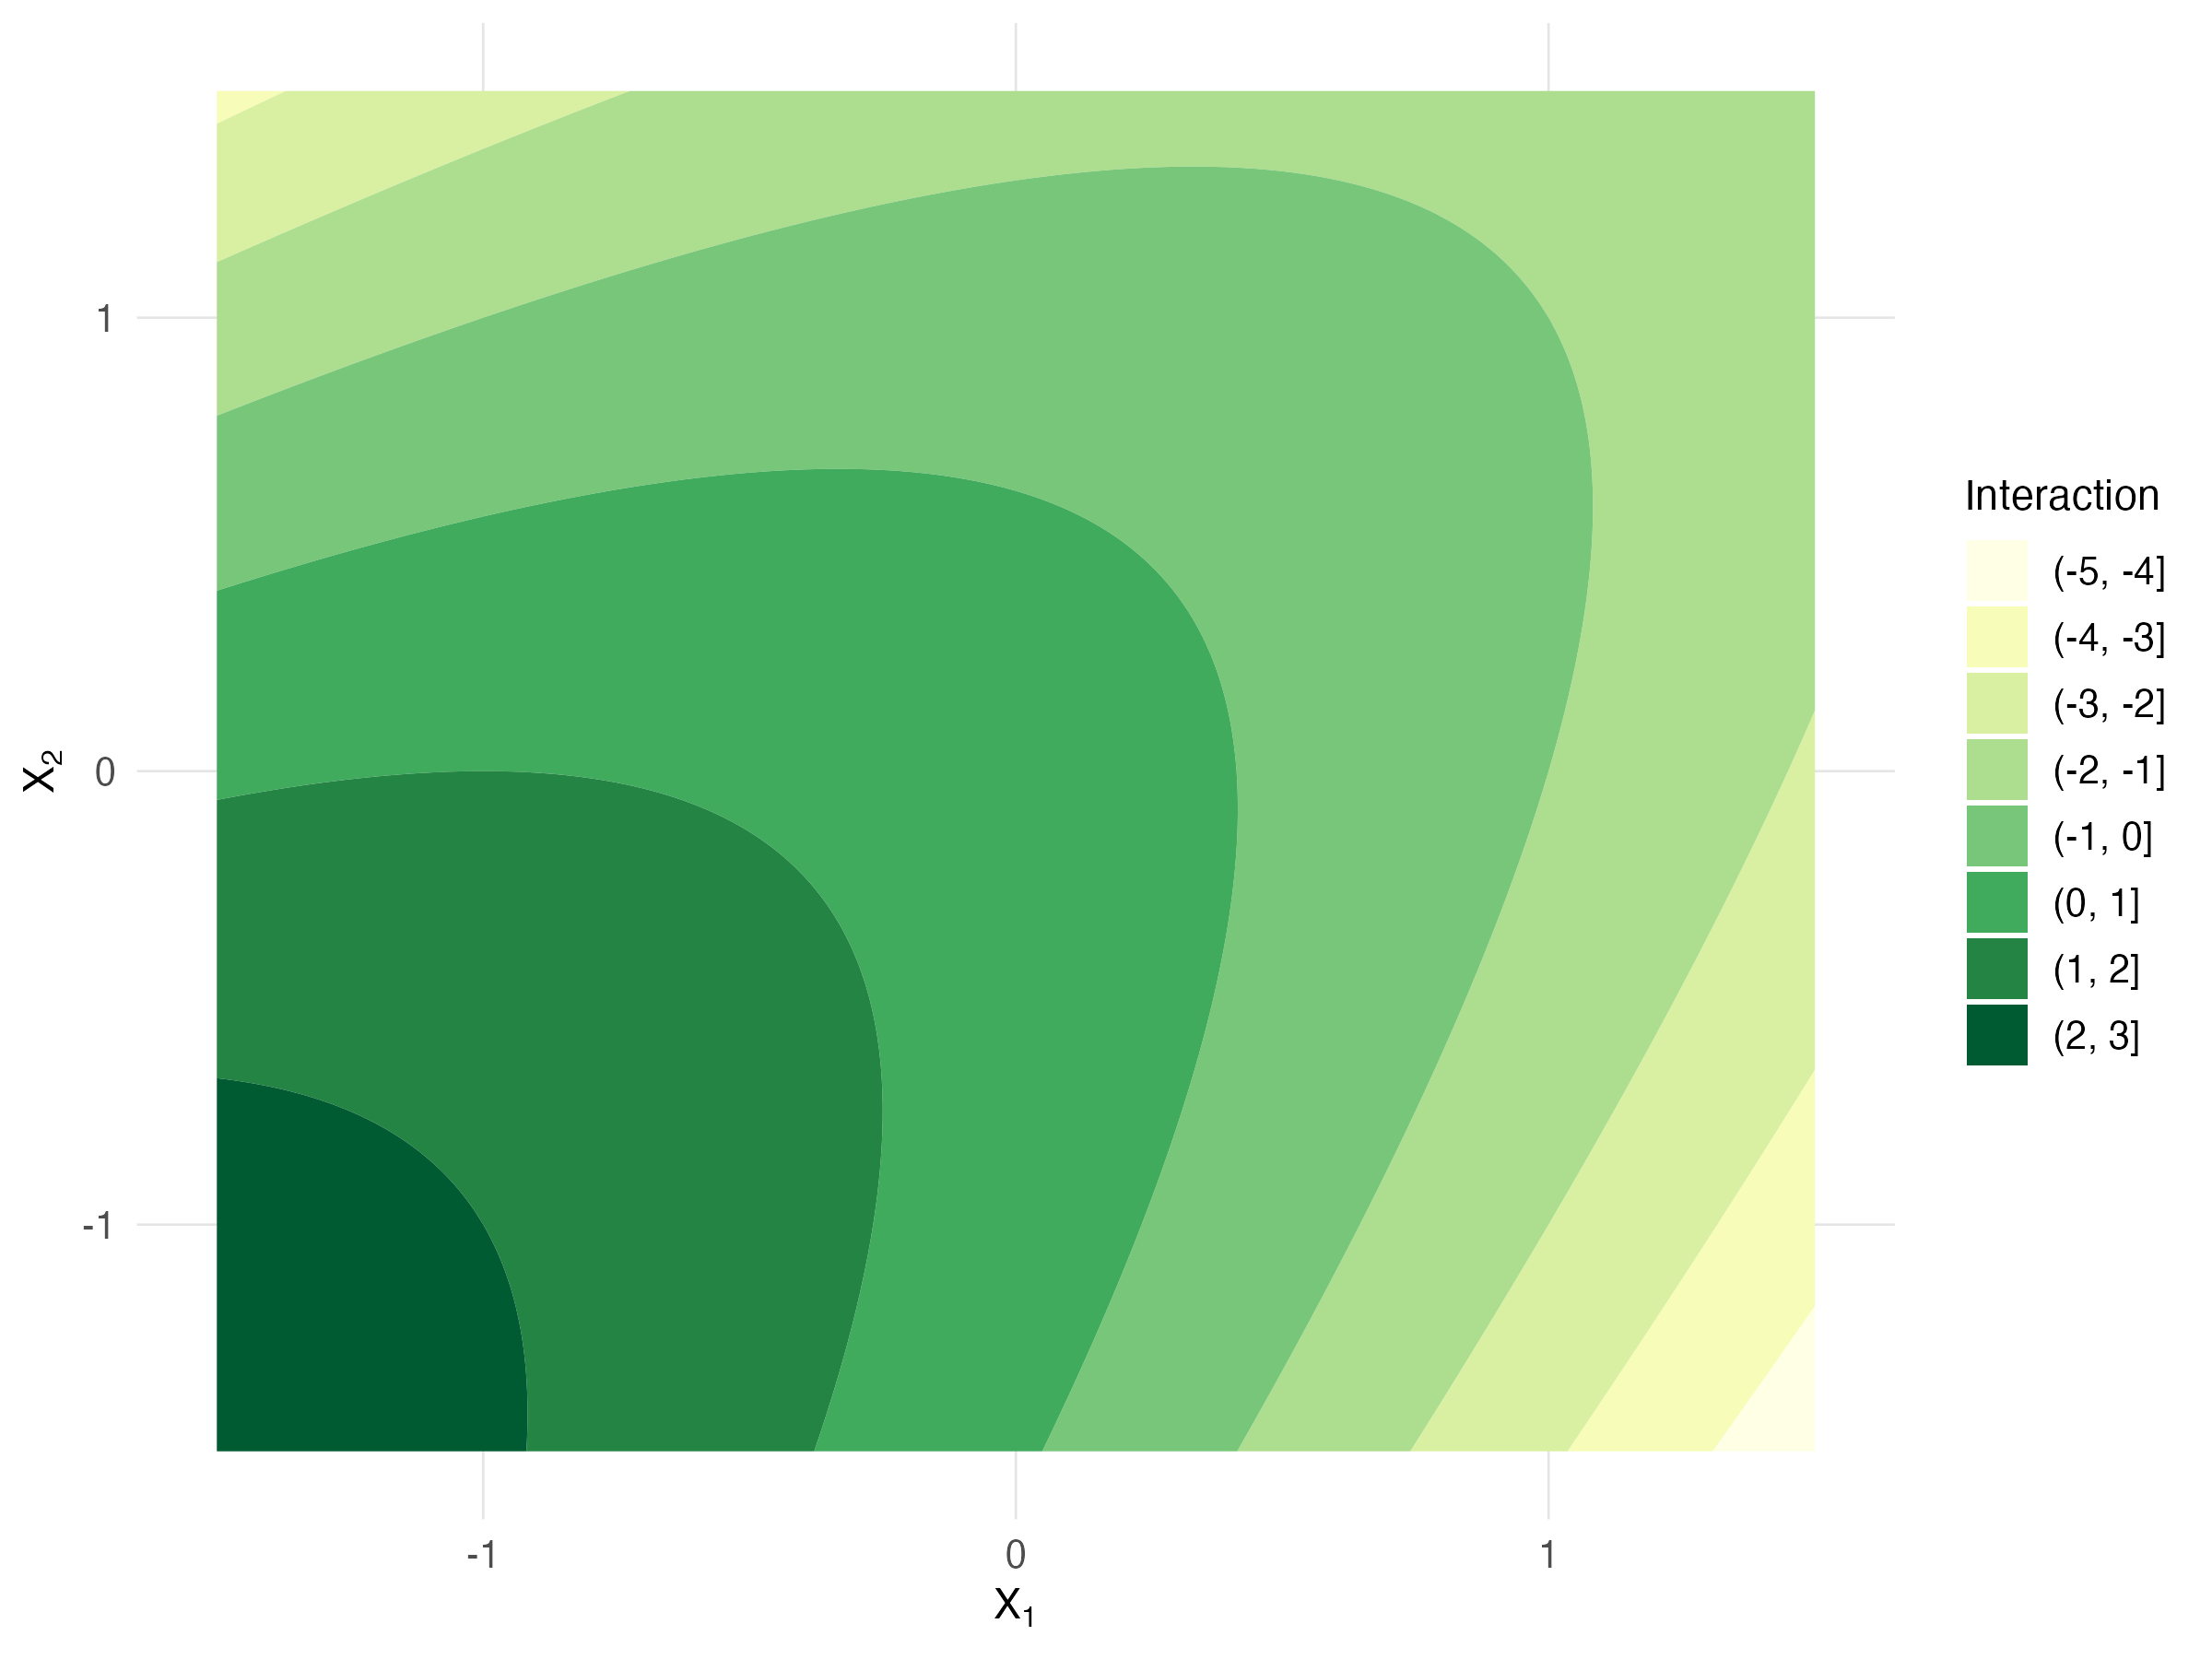
\includegraphics[width=\textwidth]{images/experiment_section/hoeffding_rho05_interaction.png}
    \end{subfigure}
    \caption{Main effects (left) and interaction effect (right) of an ANOVA-type decomposition for $g(x_1, x_2) = x_1 + 2 x_2 + x_1 x_2$ with dependent inputs, $\rho = 0.5$.}
    \label{fig:hoeffding_rho05}
\end{figure}
The true fANOVA components under $\rho = 0.5$ are given by:
\begin{align*}
y_0 &= 0.5, \\[3pt]
y_1(x_1) &= x_1 + 0.4\,(x_1^2 - 1)
        = x_1 + 0.4x_1^2 - 0.4, \\[3pt]
y_2(x_2) &= 2x_2 + 0.4\,(x_2^2 - 1)
        = 2x_2 + 0.4x_2^2 - 0.4, \\[3pt]
y_{12}(x_1,x_2) 
&= -\Big( 0.4(x_1^2 + x_2^2) - x_1 x_2 - 0.3 \Big) \\[3pt]
&= -0.4x_1^2 - 0.4x_2^2 + x_1 x_2 + 0.3.
\end{align*}
These are visualized in \autoref{fig:running_ex_dependent}.
% Input: MVN, dependent, rho = 0.5
\begin{figure}[htpb]
    \centering
    \begin{subfigure}[t]{0.49\textwidth}
        \centering
        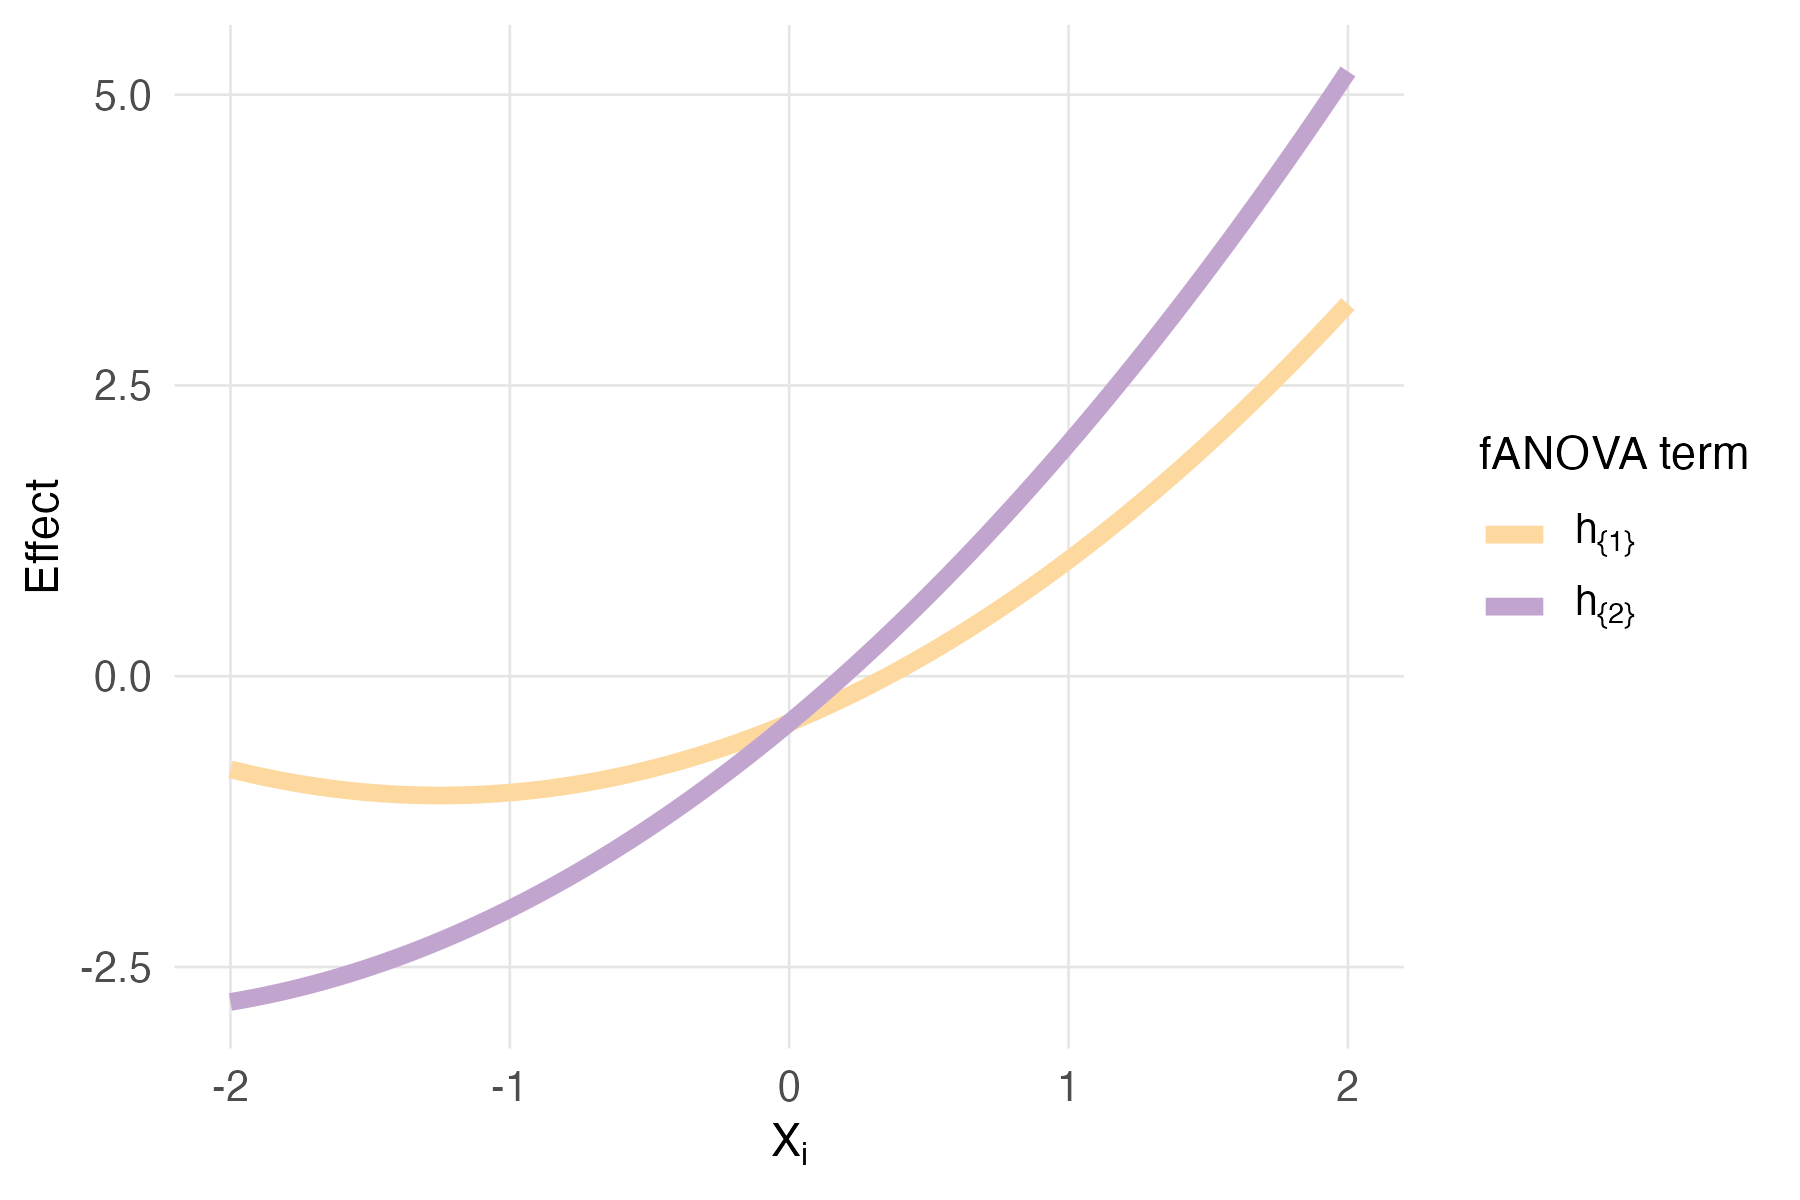
\includegraphics[width=\textwidth]{images/experiment_section/running_example_a1p10_a2p20_a11p00_a22p00_a12p10_rhop05_main.png}
    \end{subfigure}%
    \hfill
    \begin{subfigure}[t]{0.49\textwidth}
        \centering
        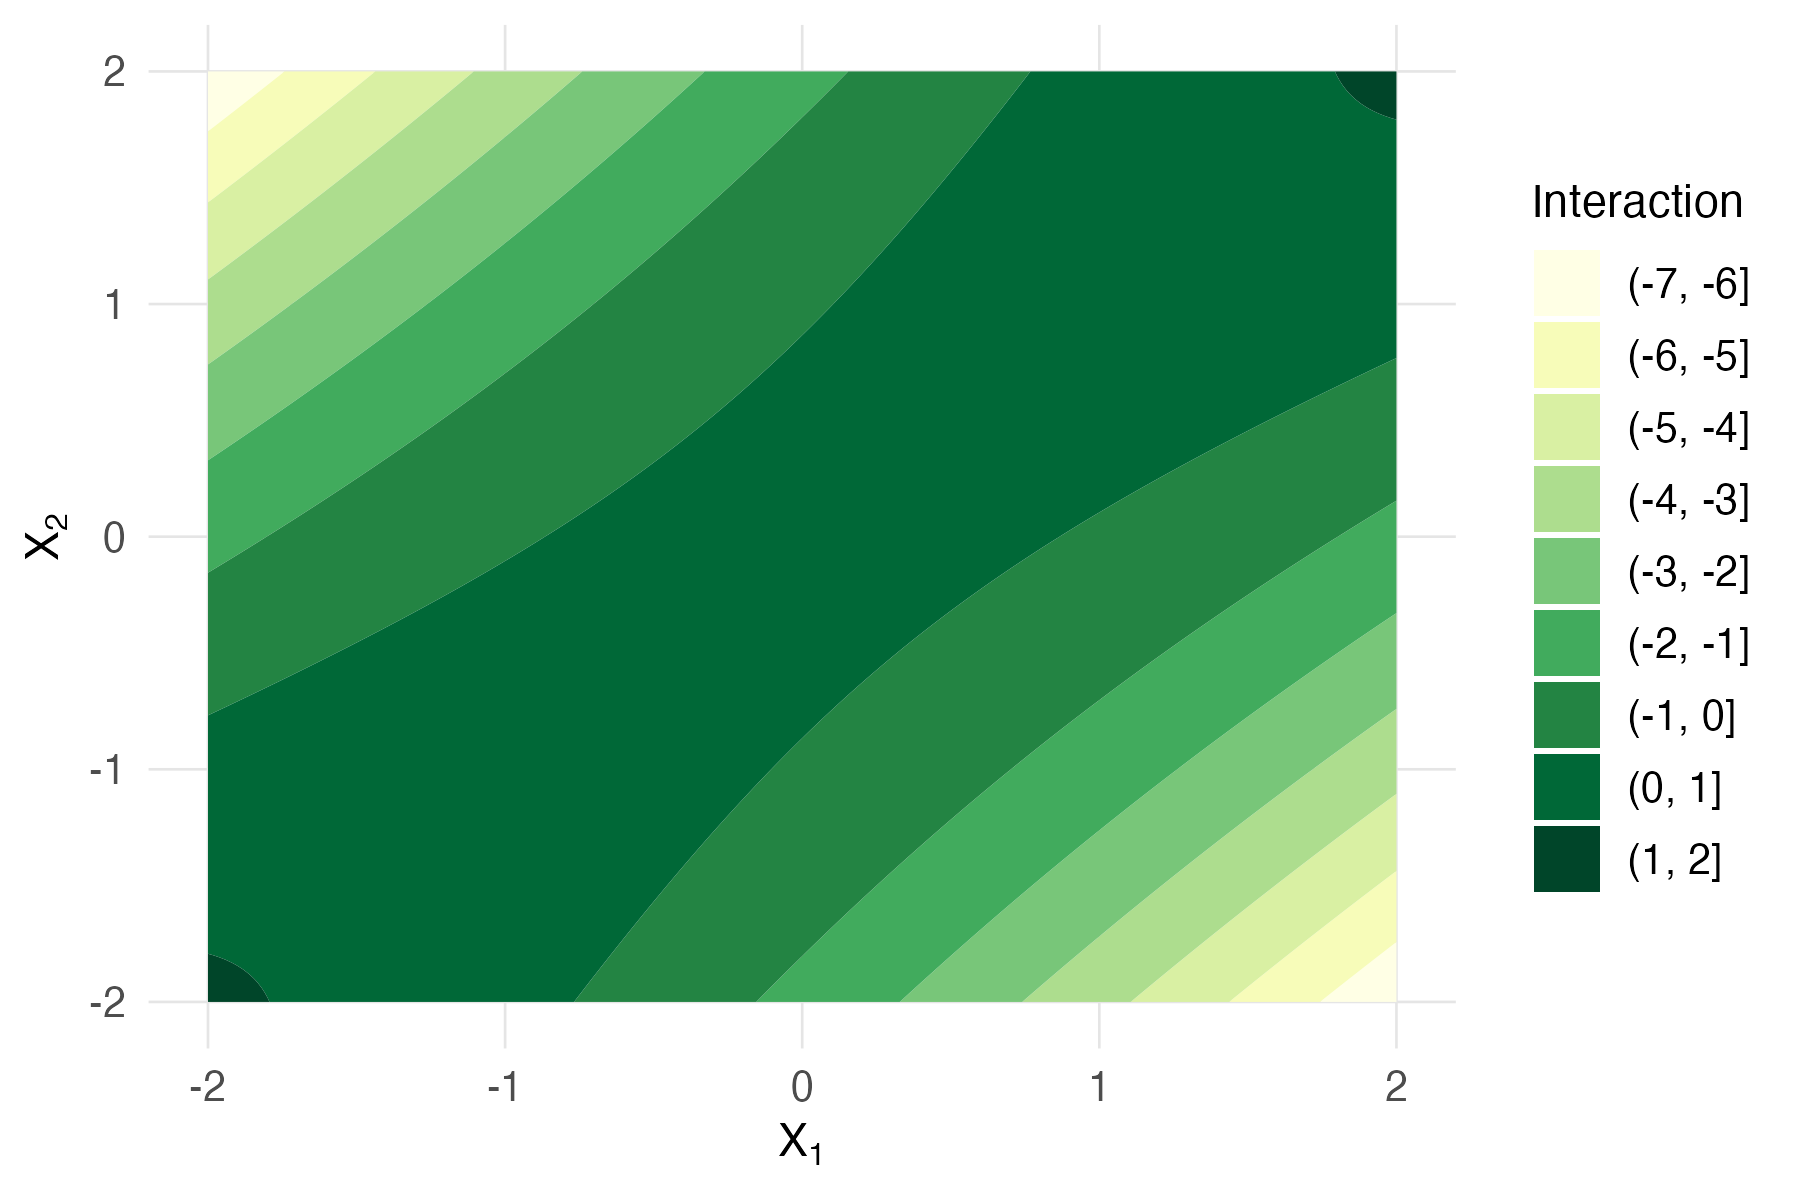
\includegraphics[width=\textwidth]{images/experiment_section/running_example_a1p10_a2p20_a11p00_a22p00_a12p10_rhop05_interaction.png}
    \end{subfigure}
    \caption{Main effects (left) and interaction effect (right) of the generalized fANOVA decomposition for $g(x_1, x_2) = x_1 + 2 x_2 + x_1 x_2$ with dependent inputs, $\rho = 0.5$.}
    \label{fig:running_ex_dependent}
\end{figure}
Interestingly, the parabolic form of the main effects is similar between both decompositions, but the interaction effects diverge notably.\par
Our running example included linear effects of both input variables and the interaction term. For the remainder of this section, we will explore other representative scenarios, we can build within the scaffold of a bivariate two degree polynomial.

\subsection{Comparison of Functions}
\subsubsection{Scenario: Linear}
First, we consider two-degree polynomials of the form:
$$g_1(x_1, x_2) = a_1 x_1 + a_2 x_2.$$
We can immediately read of the fANOVA components or use the general set of fANOVA components for a two degree polynomial in \autoref{eq:fanova_components_2D_polynomial} which simplify for $g_1$ to:
\begin{align*}
    y_1(x_1) &= a_1 x_1, \\
    y_2(x_2) &= a_2 x_2.
\end{align*}
The function $g_1$ can solely be described by linear main effects (\autoref{fig:linear_main_effects}). Since no interaction effect is present varying $\rho$ has no impact on the main effects.

\begin{figure}[htpb]
    \centering
    \begin{subfigure}[t]{0.49\textwidth}
        \centering
        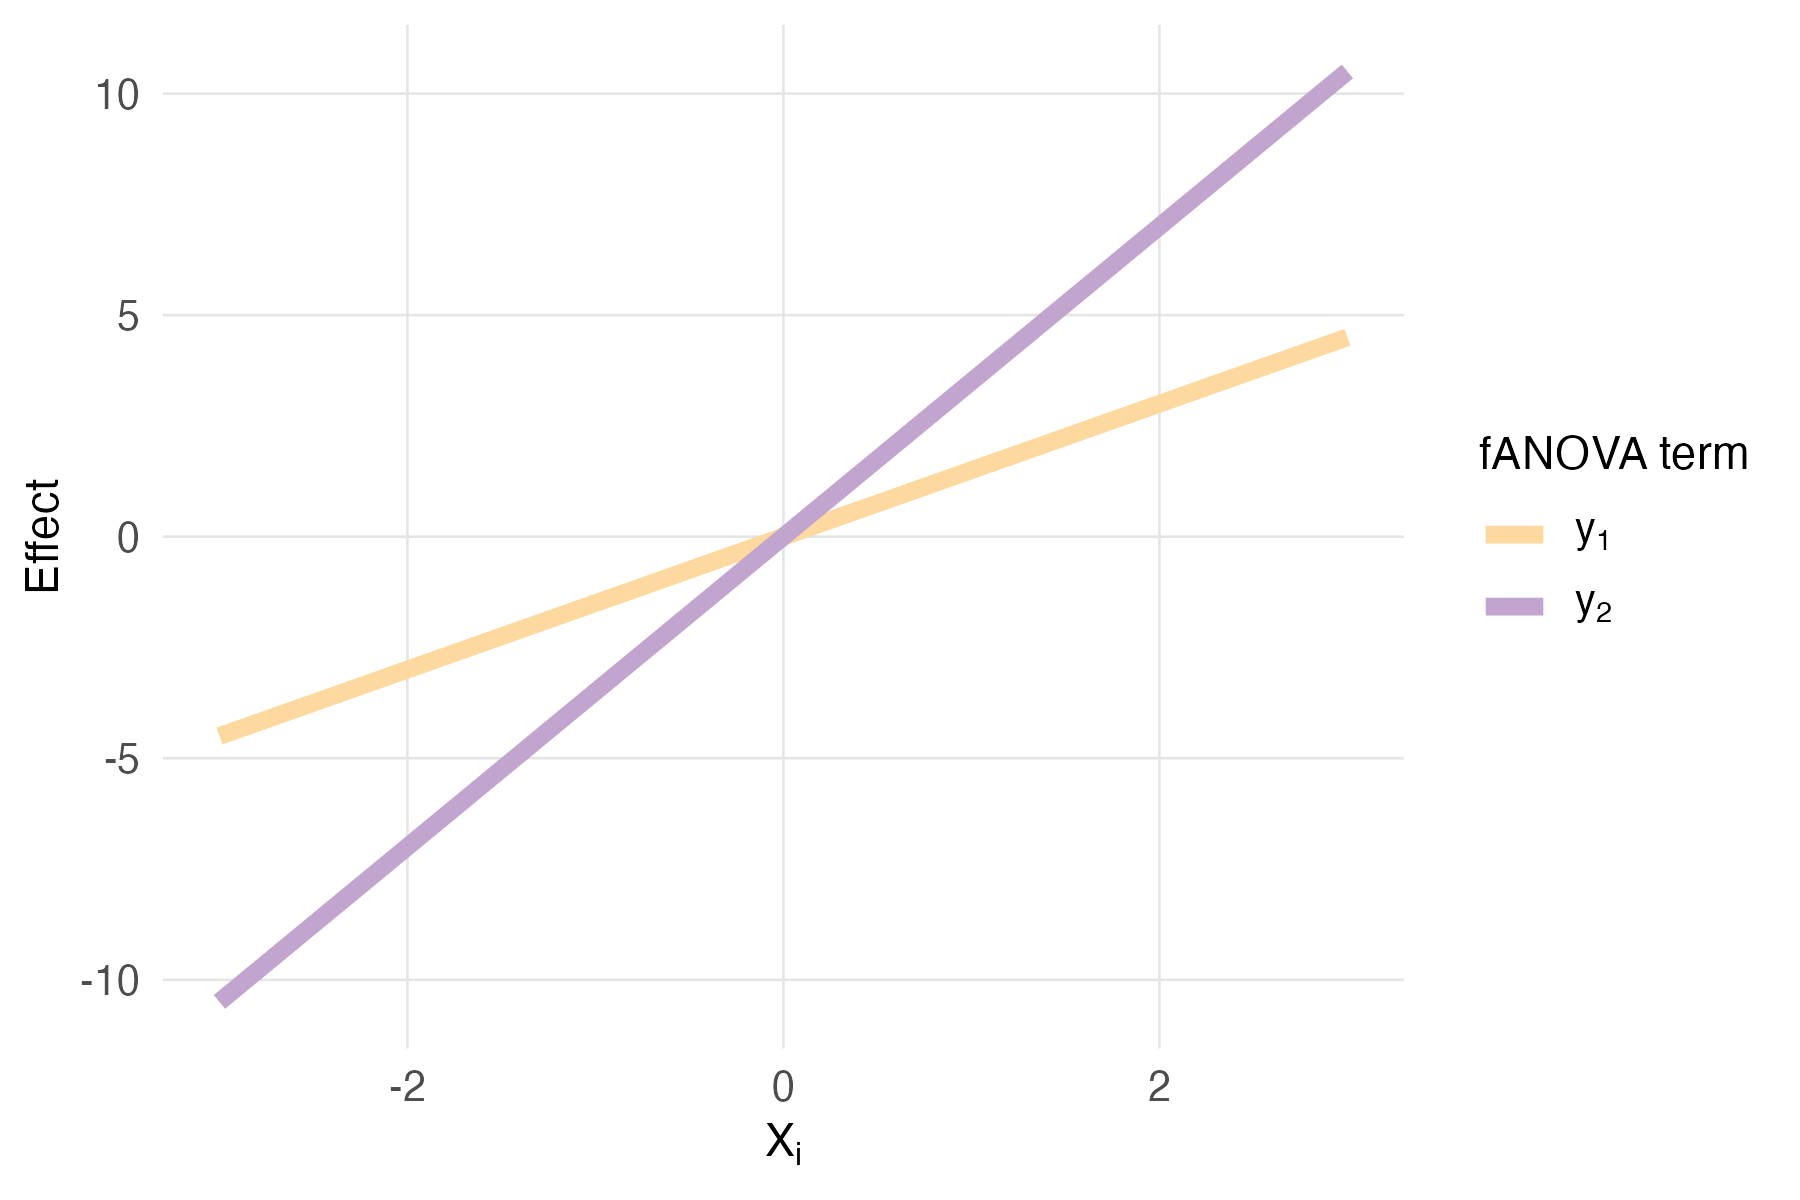
\includegraphics[width=\textwidth]{images/experiment_section/linear_a1p15_a2p35_a11p00_a22p00_a12p00_rhop00_main.png}
        \caption{$a_1 = 1.5$, $a_2 = 3.5$}
    \end{subfigure}%
    \hfill
    \begin{subfigure}[t]{0.49\textwidth}
        \centering
        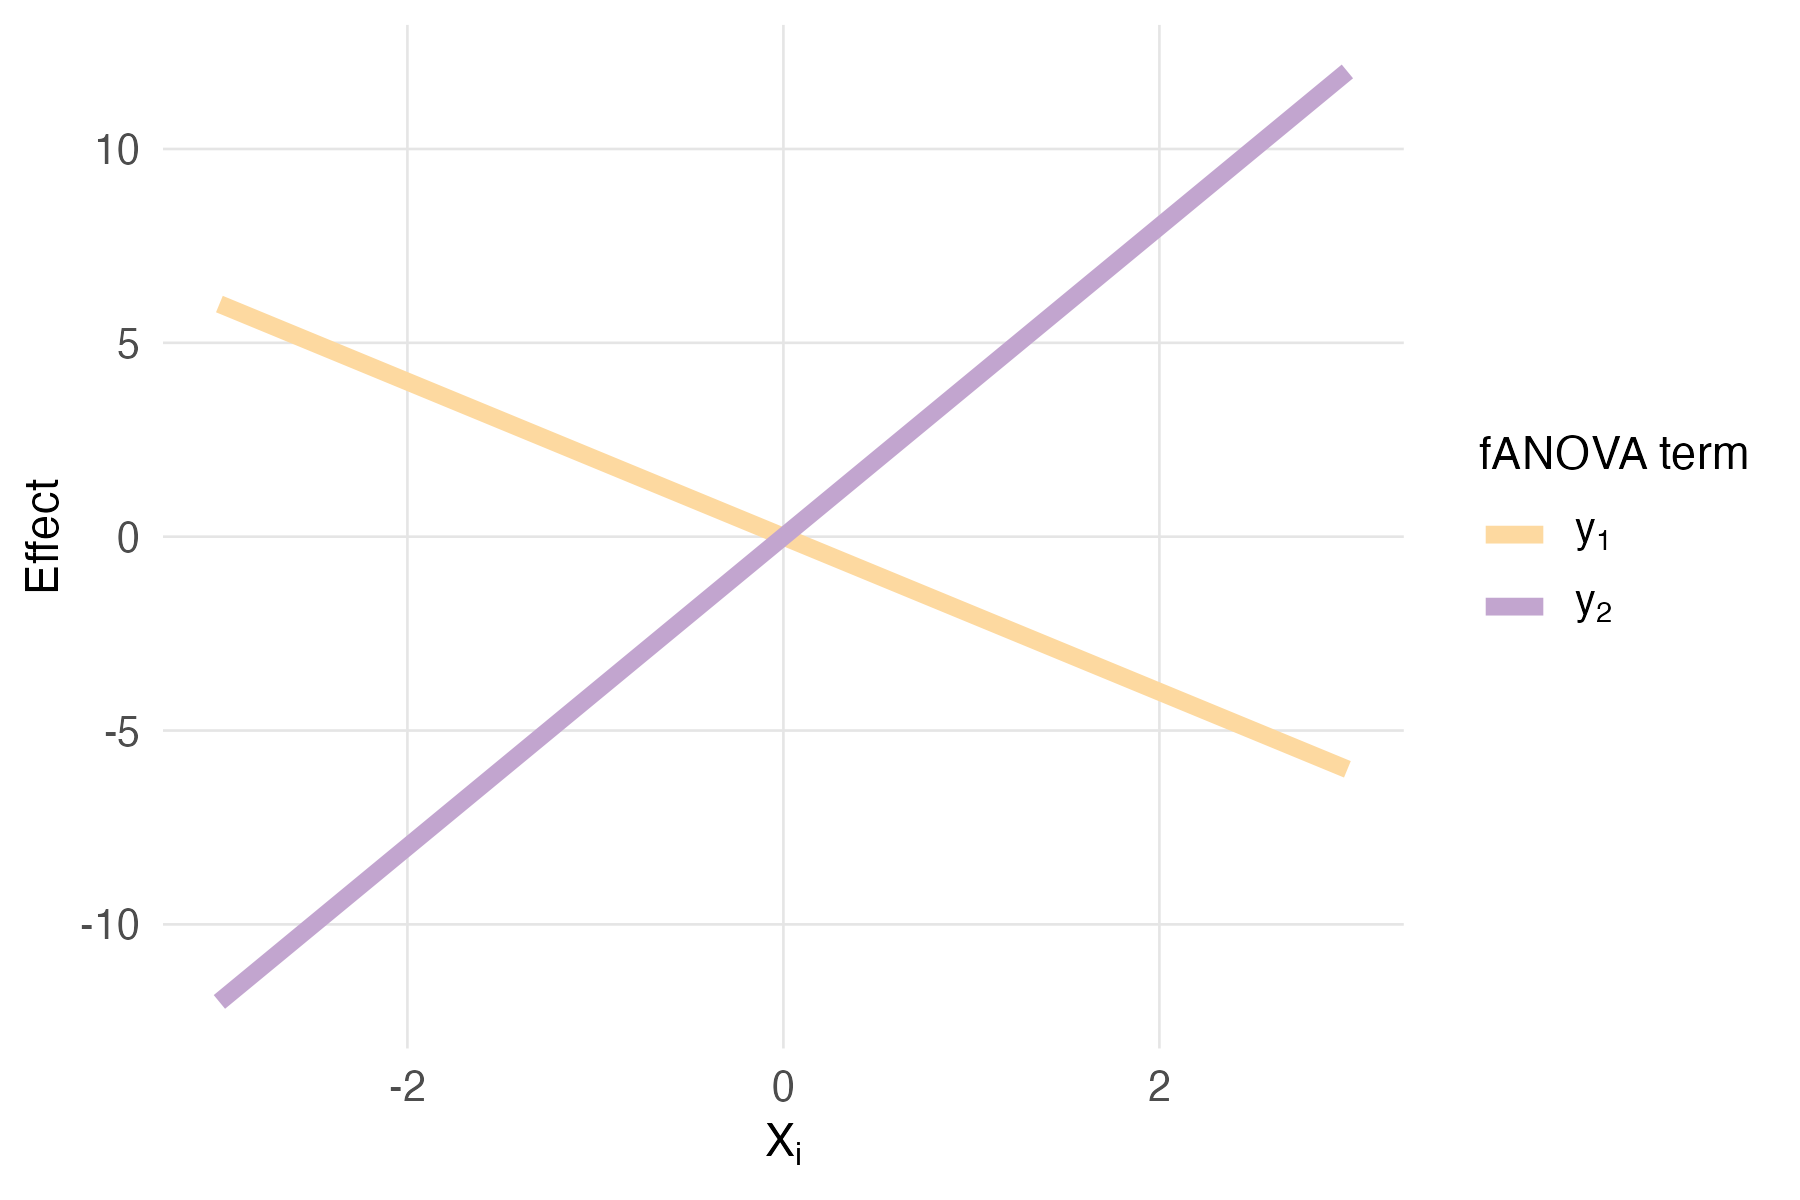
\includegraphics[width=\textwidth]{images/experiment_section/linear_a1m20_a2p40_a11p00_a22p00_a12p00_rhop00_main.png}
        \caption{$a_1 = -2$, $a_2 = 4$}
    \end{subfigure}
    \caption{Main fANOVA components for linear terms with different coefficients. The components are given by: $y_1(x_1) = a_1 x_1$, $y_2(x_2) = a_2 x_2$.}
    \label{fig:linear_main_effects}
\end{figure}


\subsubsection{Scenario: Linear and Quadratic}
Slightly more complex is a two-degree polynomials, which allow for effects of linear and quadratic nature:
\[
g_2(x_1, x_2) = a_1 x_1 + a_2 x_2 + a_{11} x_1^2 + a_{22} x_2^2.
\]
The fANOVA components for $g_4$ are given by:
\begin{align*}
    y_{\emptyset} &= a_{11} + a_{22}, \\
    y_1(x_1) &= a_1 x_1 + a_{11}(x_1^2 - 1), \\
    y_2(x_2) &= a_2 x_2 + a_{22}(x_2^2 - 1).
\end{align*}
The main effects are parabolas now. In \autoref{fig:mixed_main_effects}, we vary the coefficients $a_1$, $a_2$, $a_{11}$, and $a_{22}$, while the interaction term is still absent.
% The shape of the parabolas in the upper left panel is representative of cases, where the coefficients of the linear terms $a_1$ and $a_2$ have the same sign and the ones of the quadratic terms $a_{11}$ and $a_{22}$ have the same sign.
The coefficients of the quadratic terms determine whether the parabola is facing downwards or upwards; when $a_{11}$ and $a_{22}$ are both negative or both positive the parabola is open downwards or upwards respectively, and when they have opposite signs the parabolas are open in different directions. Alongside the quadratic coefficients, the linear ones $a_1$ and $a_2$ influence how stretched or compressed the parabola is.

\begin{figure}[htpb]
    \centering
    % --- Row 1 ---
    \begin{subfigure}[t]{0.49\textwidth}
        \centering
        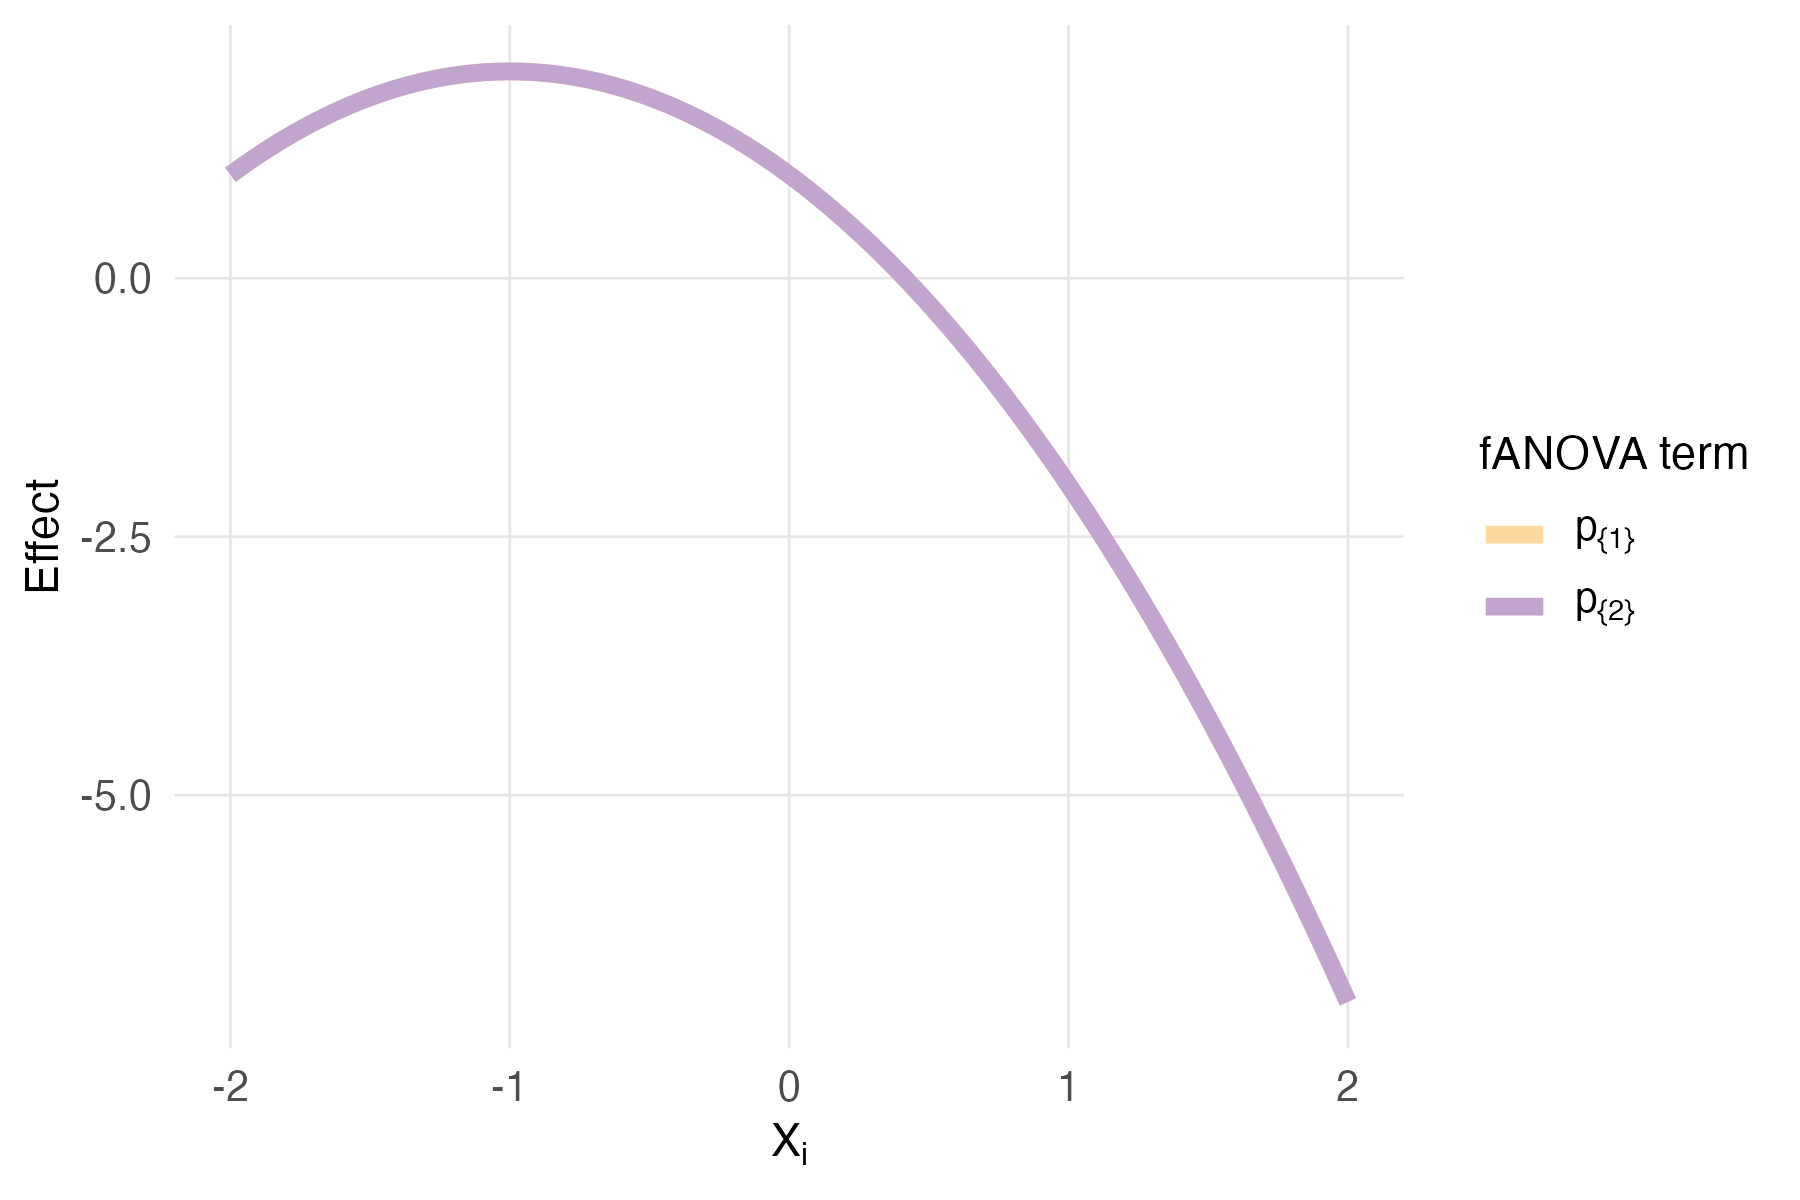
\includegraphics[width=\textwidth]{images/experiment_section/mixed_a1m20_a2m20_a11m10_a22m10_a12p00_rhop00_main.png}
        \caption{$a_1=-2,\, a_2=-2,\, a_{11}=-1,\, a_{22}=-1$}
        \label{fig:mixed_rho_0_panel1}
    \end{subfigure}%
    \hfill
    \begin{subfigure}[t]{0.49\textwidth}
        \centering
        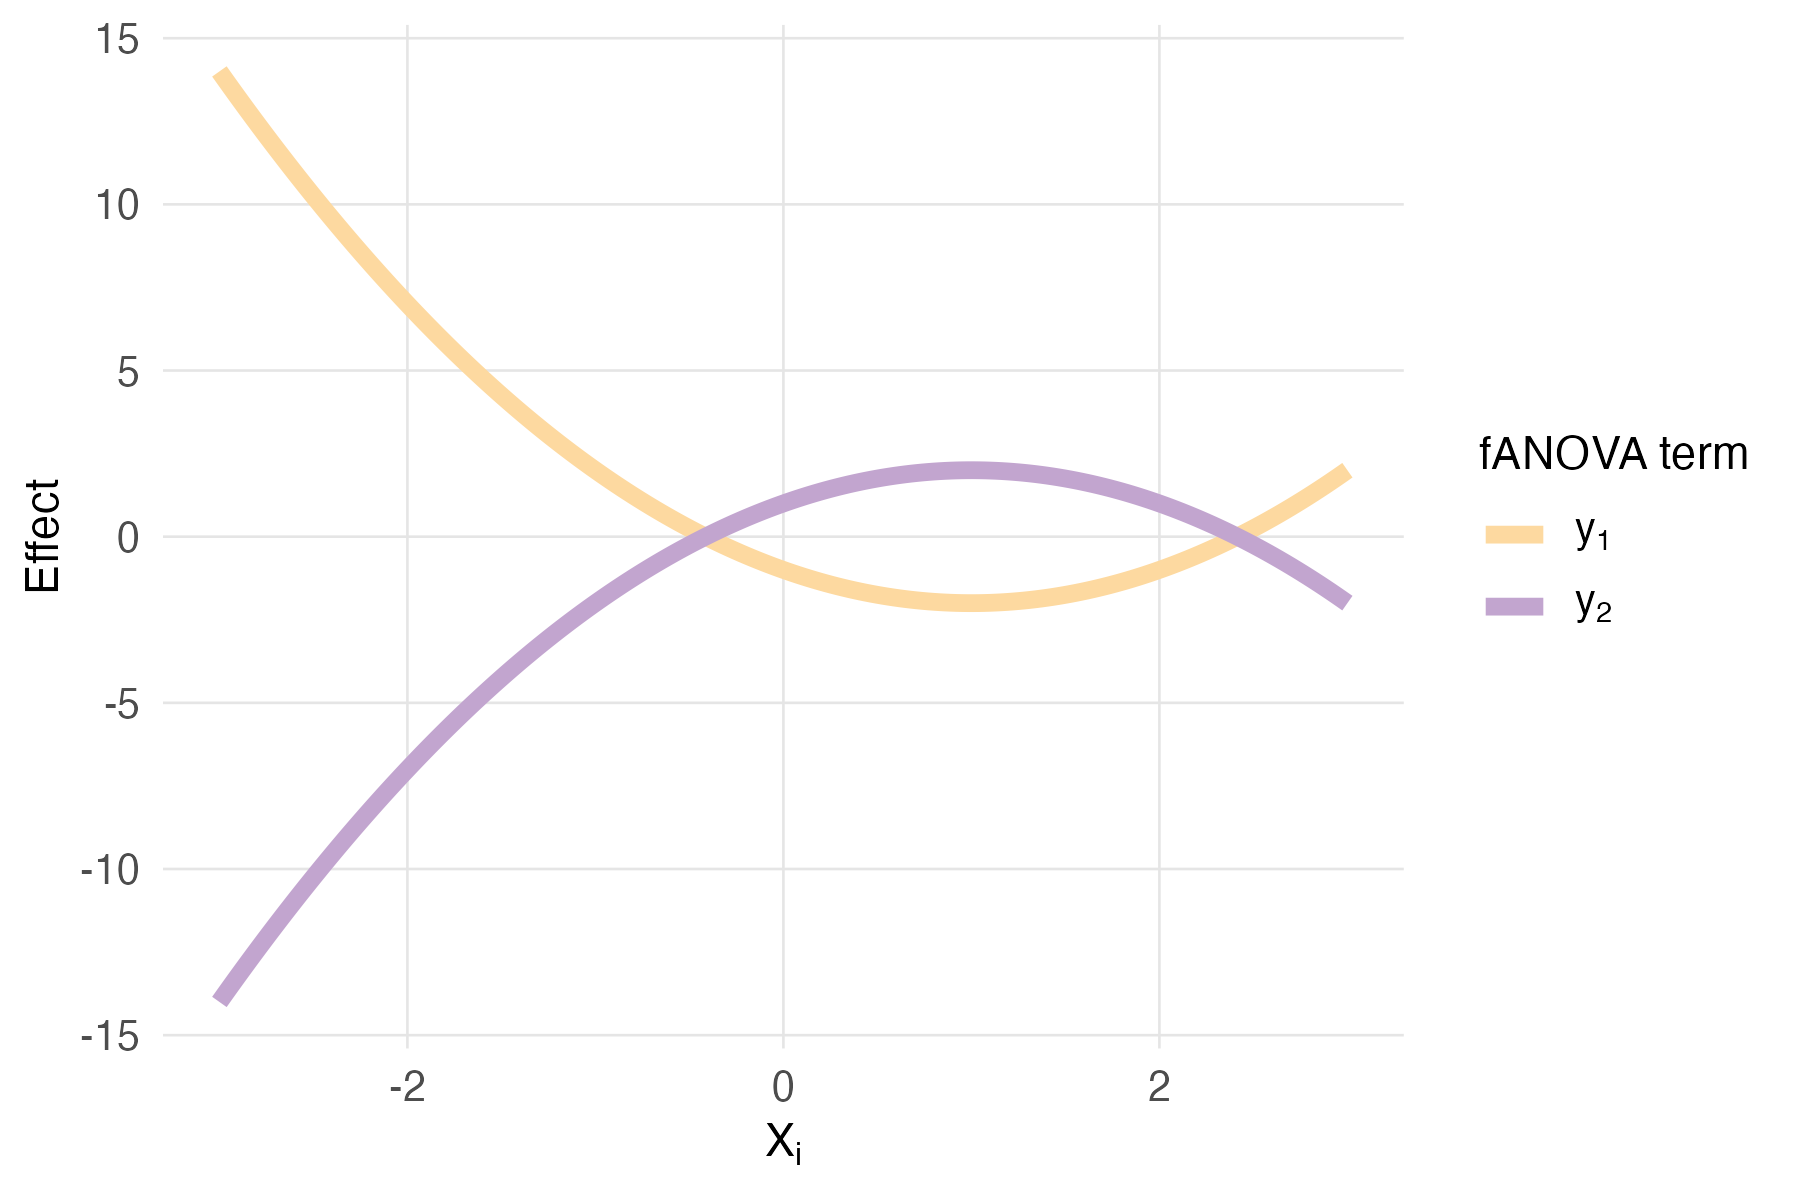
\includegraphics[width=\textwidth]{images/experiment_section/mixed_a1m20_a2p20_a11p10_a22m10_a12p00_rhop00_main.png}
        \caption{$a_1=-2,\, a_2=2,\, a_{11}=1,\, a_{22}=-1$}
        \label{fig:mixed_rho_0_panel2}
    \end{subfigure}

    % --- Row 2 ---
    \begin{subfigure}[t]{0.49\textwidth}
        \centering
        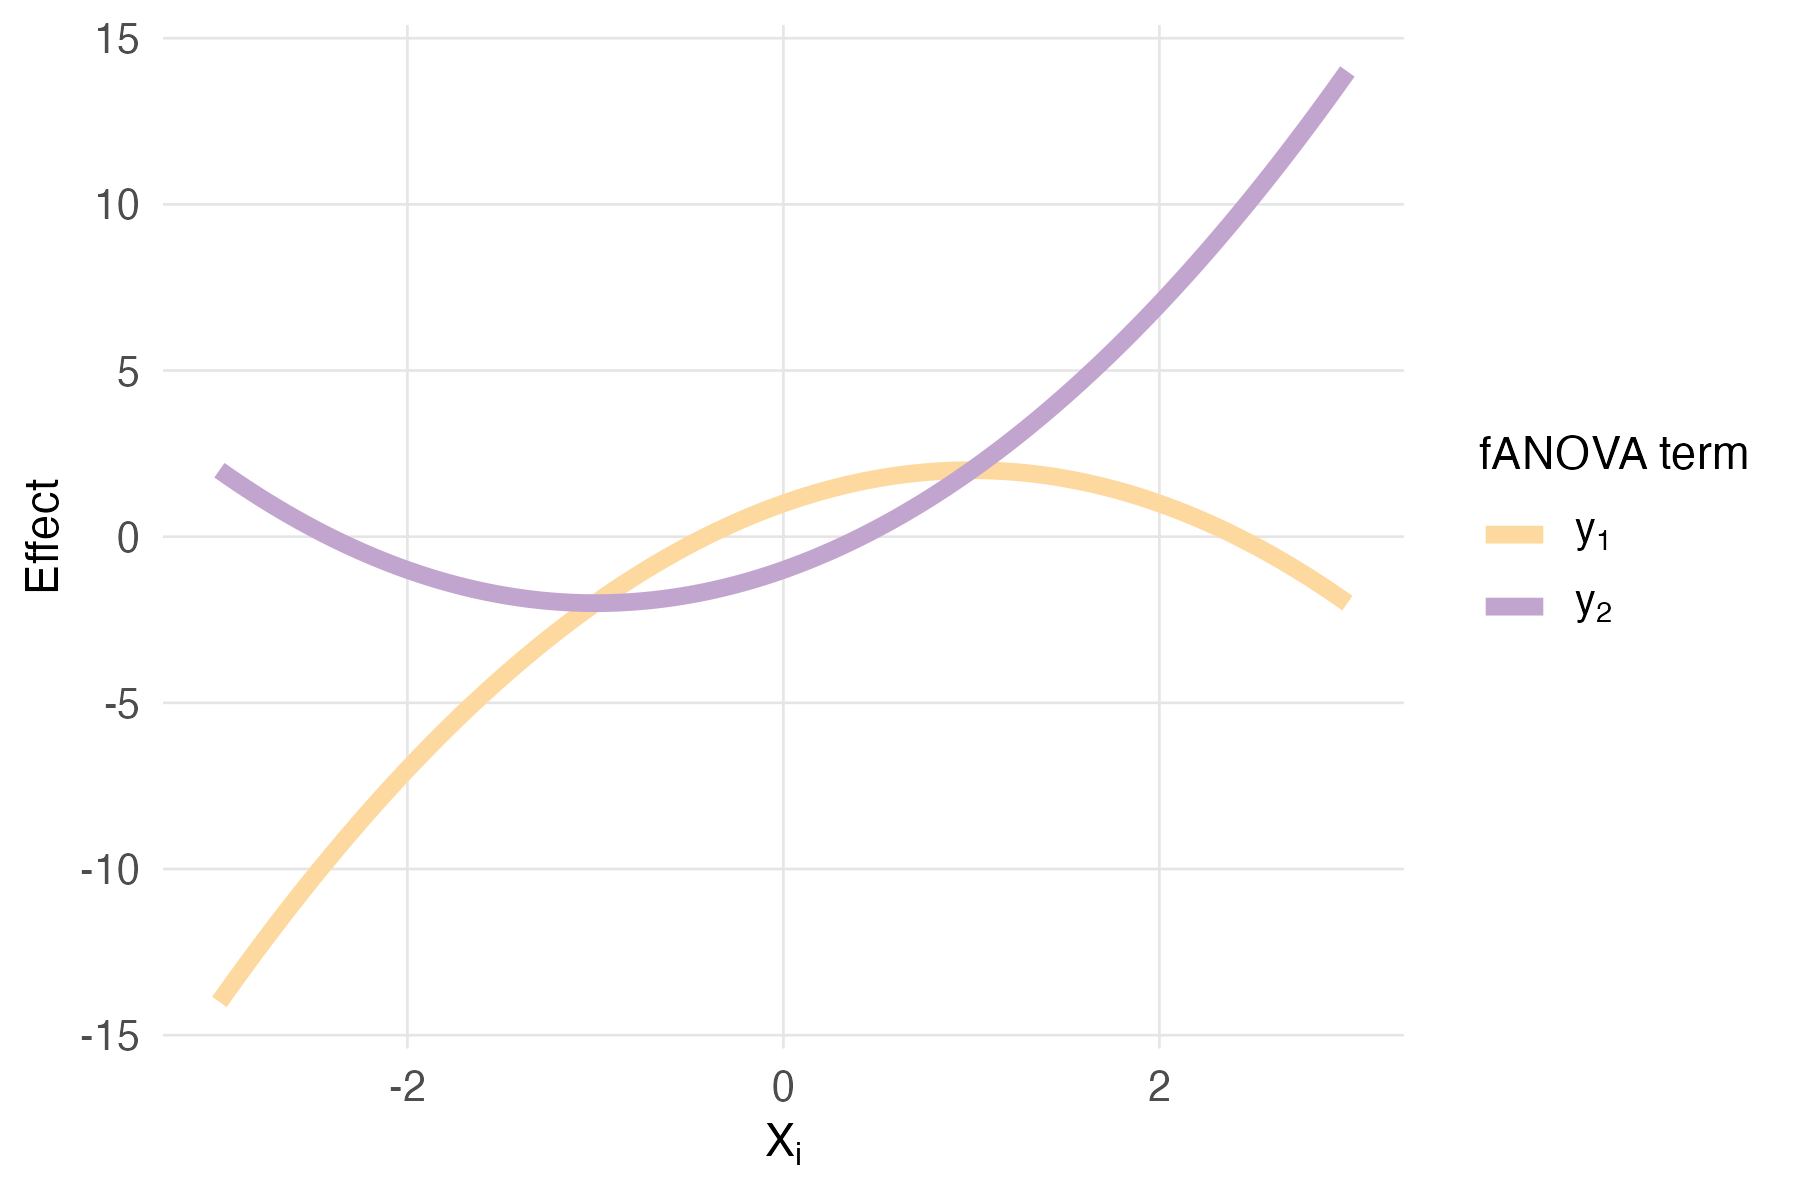
\includegraphics[width=\textwidth]{images/experiment_section/mixed_a1p20_a2p20_a11m10_a22p10_a12p00_rhop00_main.png}
        \caption{$a_1=2,\, a_2=2,\, a_{11}=-1,\, a_{22}=1$}
        \label{fig:mixed_rho_0_panel3}
    \end{subfigure}%
    \hfill
    \begin{subfigure}[t]{0.49\textwidth}
        \centering
        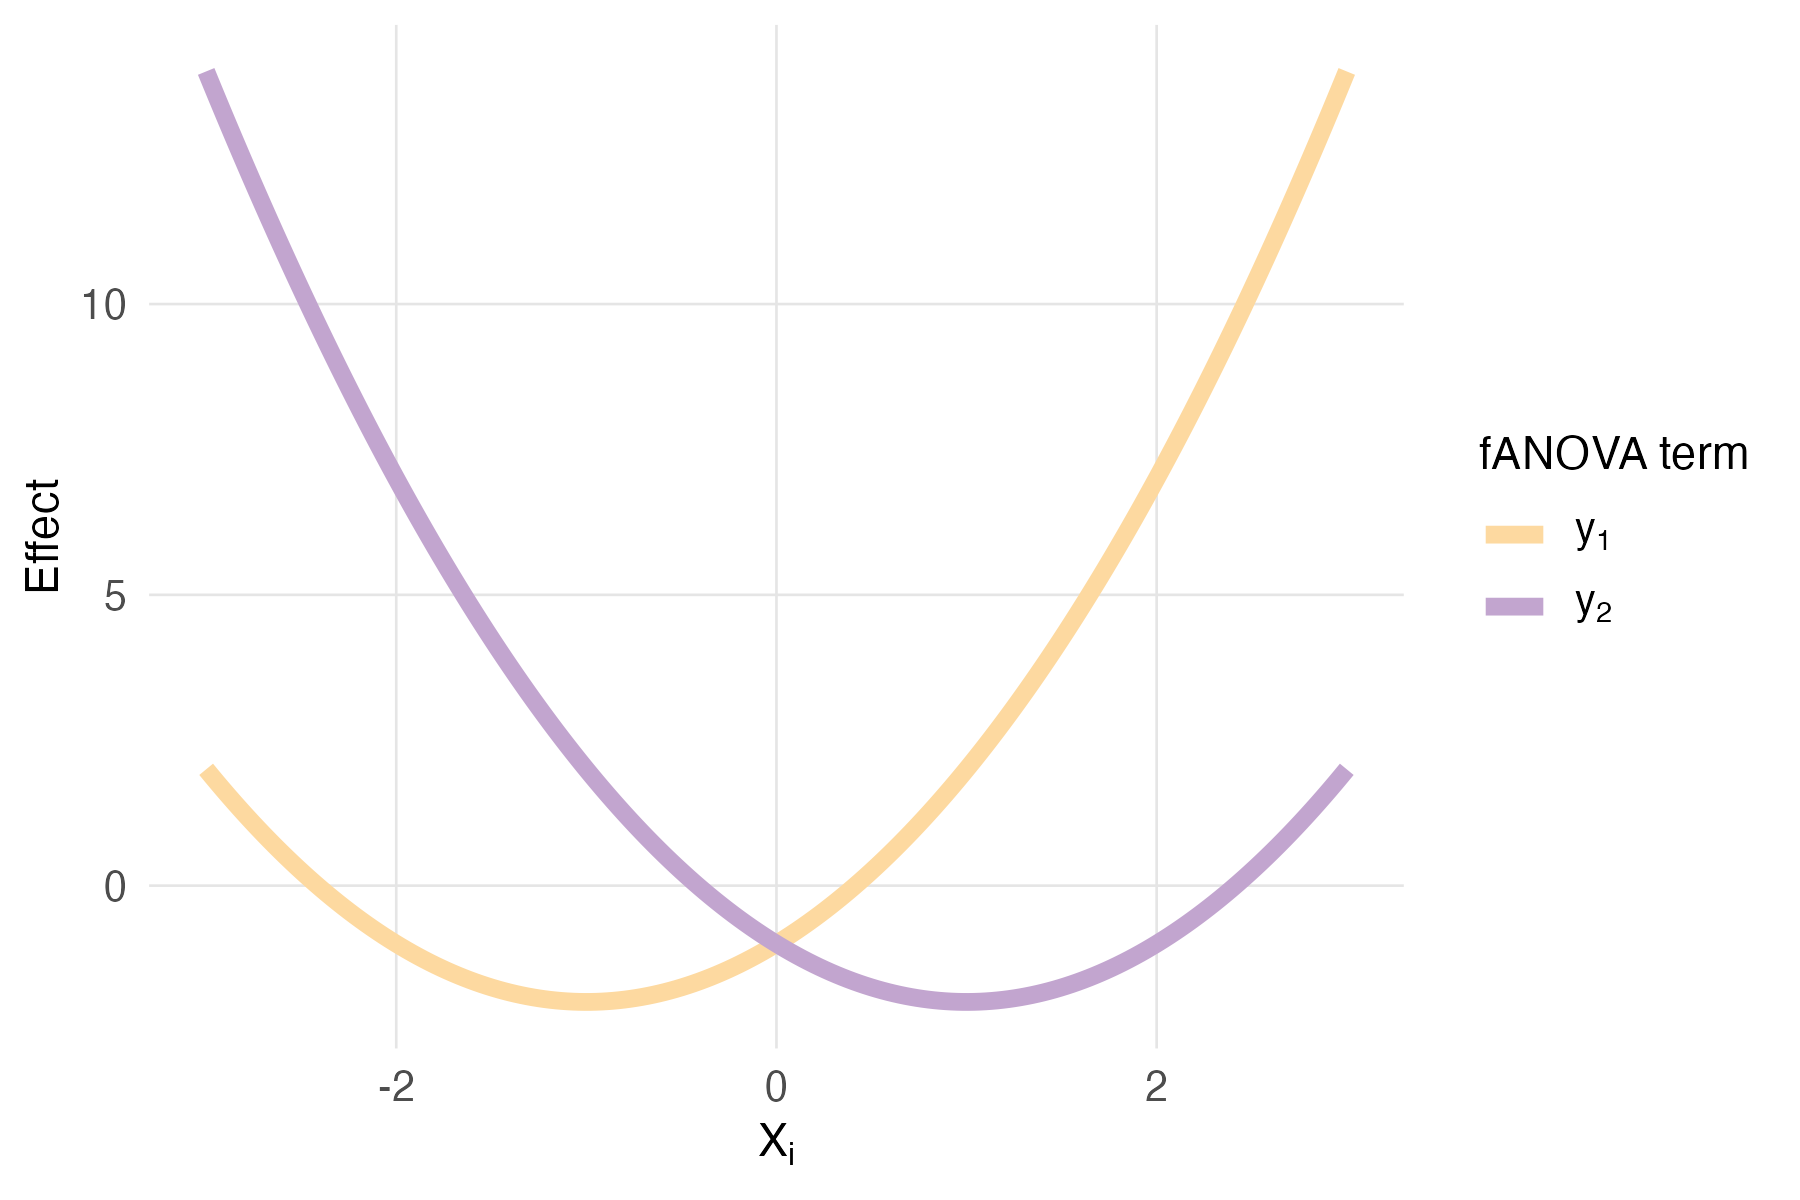
\includegraphics[width=\textwidth]{images/experiment_section/mixed_a1p20_a2m20_a11p10_a22p10_a12p00_rhop00_main.png}
        \caption{$a_1=2,\, a_2=-2,\, a_{11}=1,\, a_{22}=1$}
        \label{fig:mixed_rho_0_panel4}
    \end{subfigure}

    \caption{Main effects for different coefficient combinations of mixed main effects. The commponents are given by: $y_1(x_1) = a_1 x_1 + a_{11}(x_1^2 - 1)$, $y_2(x_2) = a_2 x_2 + a_{22}(x_2^2 - 1)$.}
    \label{fig:mixed_main_effects}
\end{figure}

\subsubsection{Scenario: Interaction}
Next, we consider a model, which solely consists of an interaction term:
$$g_3(x_1, x_2) = a_{12} x_1 x_2.$$
The fANOVA components for $g_3$ are given by:
\begin{align*}
    y_{\emptyset} &= a_{12} \rho, \\
    y_{1}(x_1) &= a_{12} \frac{\rho}{1+ \rho} (x_1^2 - 1), \\
    y_{2}(x_2) &= a_{12} \frac{\rho}{1+ \rho} (x_2^2 - 1), \\
    y_{12}(x_1,x_2) 
&= -a_{12}\!\left(
    \frac{\rho(x_1^2+x_2^2)}{1+\rho^2} 
    - x_1 x_2 
    + \frac{\rho(\rho^2-1)}{1+\rho^2}
   \right).
\end{align*}
The main effects $y_1$ and $y_2$, as well as the interaction term $y_{12}$, are influenced by $\rho$ and $a_{12}$.
In our example we keep $a_{12} = 2$ fixed and show the interaction effect as a contour plot for varying $\rho$ with the corresponding main effects next to it \autoref{fig:interaction_combined}.
The main effects have the same form for every case of $\rho$ and $a_{12}$ and thus overlap. This example is simple yet interesting because it shows that in the case where the true function consists solely of an interaction term, fANOVA still attributes something to the isolated effect of each variable. Only when the variables are uncorrelated, all the effect is attributed to the interaction term. This functionality hints to why \cite{lengerich2020} build an algorithm around fANOVA to purify interaction effects\footnote{Because they see a pure interaction as an effect which cannot be attributed to lower order terms; this means when identifying interactions we want to attribute all we can to lower order terms and what is left is the true interaction effect.}.


\begin{figure}[htpb]
    \centering
    % ----- Row 1 -----
    \begin{subfigure}[t]{0.49\textwidth}
        \centering
        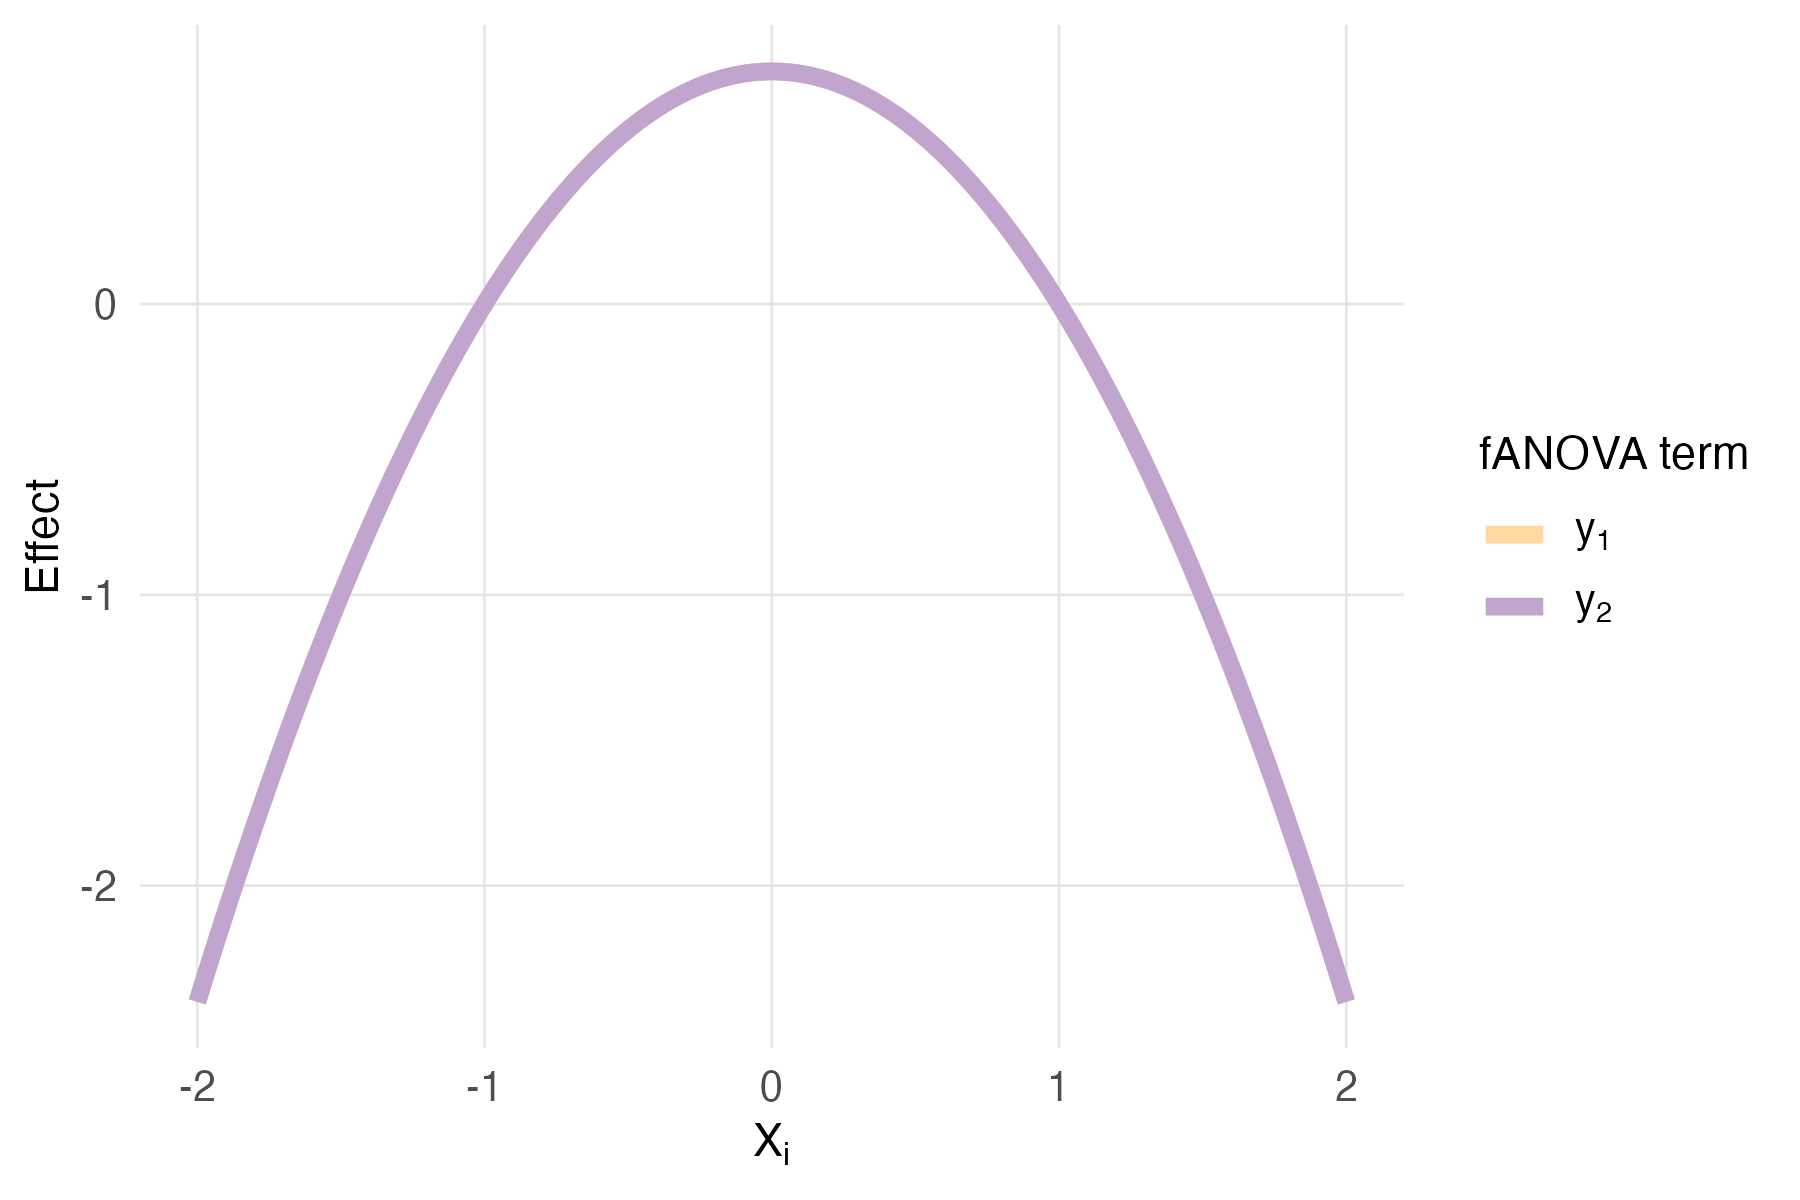
\includegraphics[width=\textwidth]{images/experiment_section/interaction_a1p00_a2p00_a11p00_a22p00_a12p20_rhom05_main.png}
        \caption{Main effects for $\rho = -0.5$}
    \end{subfigure}%
    \hfill
    \begin{subfigure}[t]{0.49\textwidth}
        \centering
        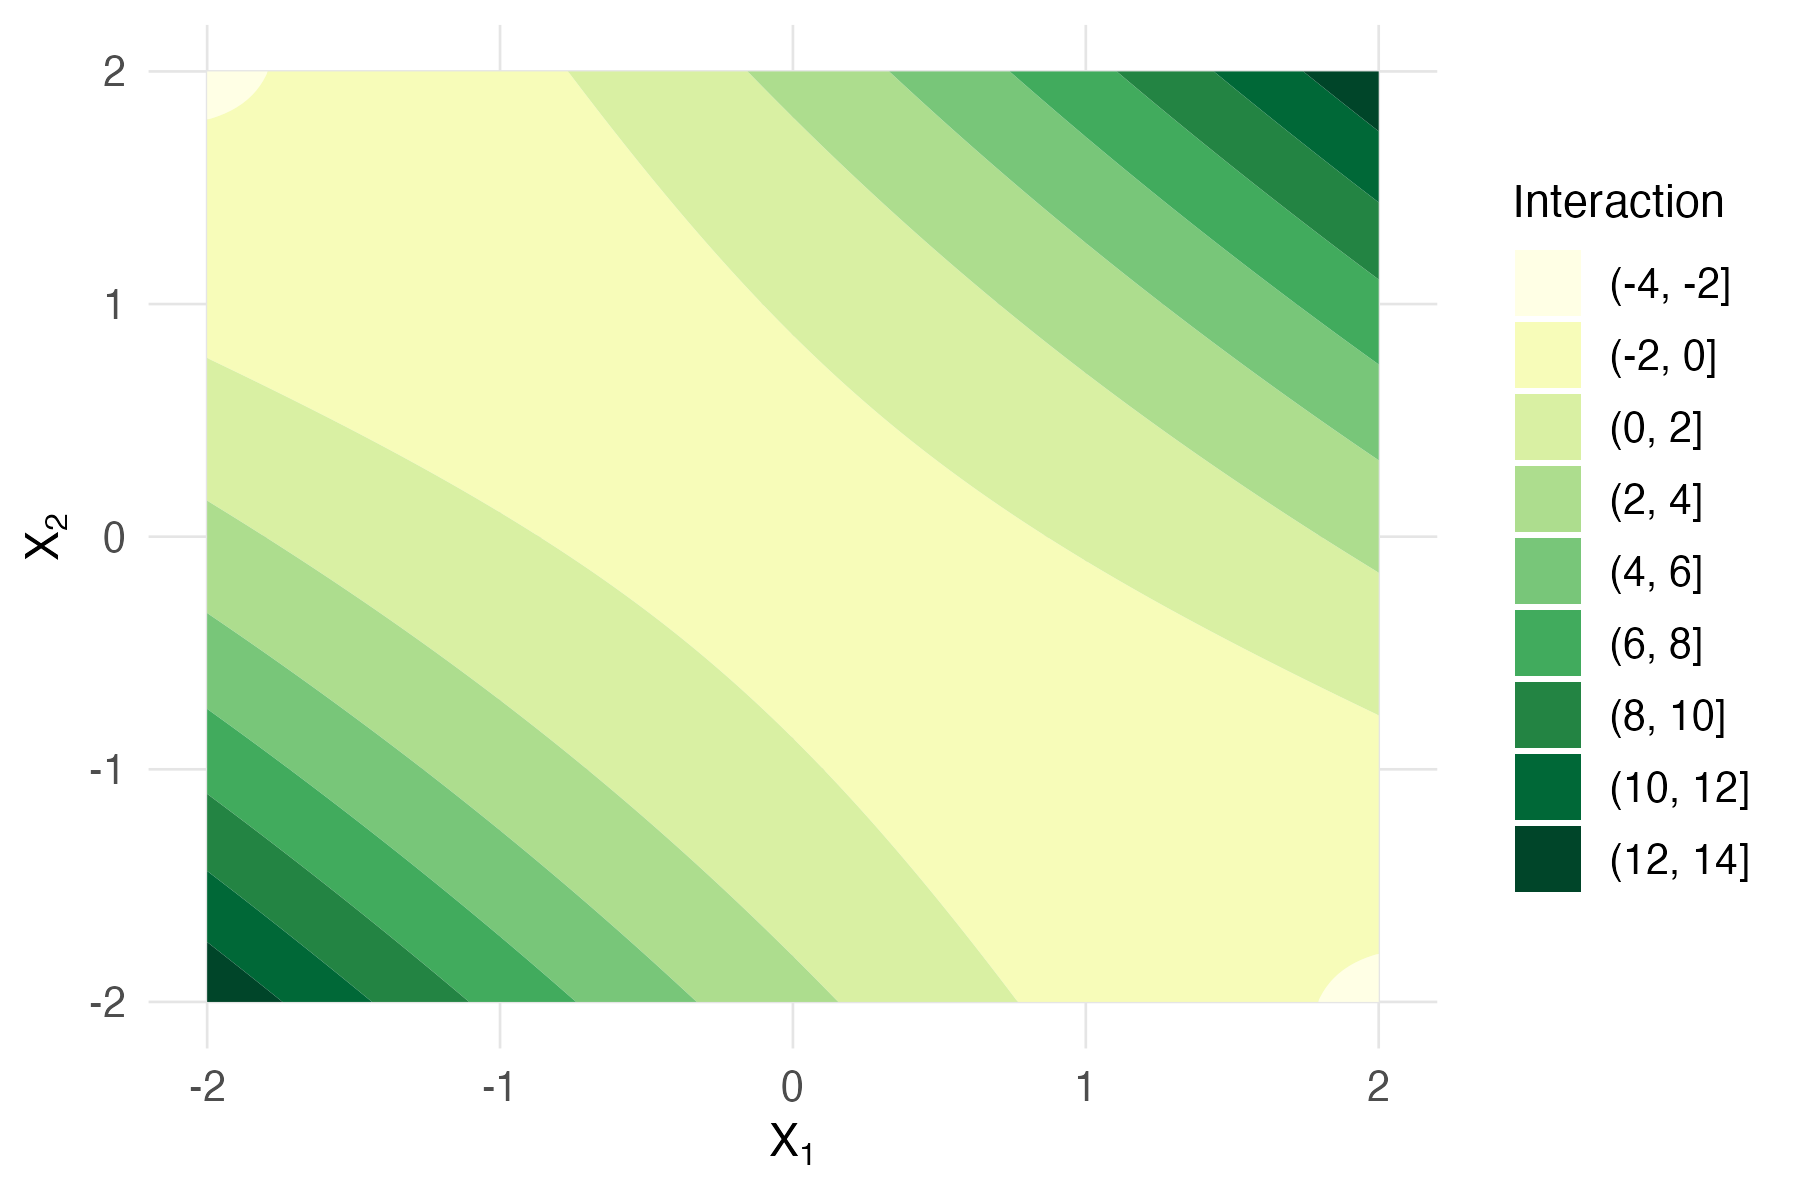
\includegraphics[width=\textwidth]{images/experiment_section/interaction_a1p00_a2p00_a11p00_a22p00_a12p20_rhom05_interaction.png}
        \caption{Interaction contour for $\rho = -0.5$}
    \end{subfigure}

    \vspace{0.5em}
    % ----- Row 2 -----
    \begin{subfigure}[t]{0.49\textwidth}
        \centering
        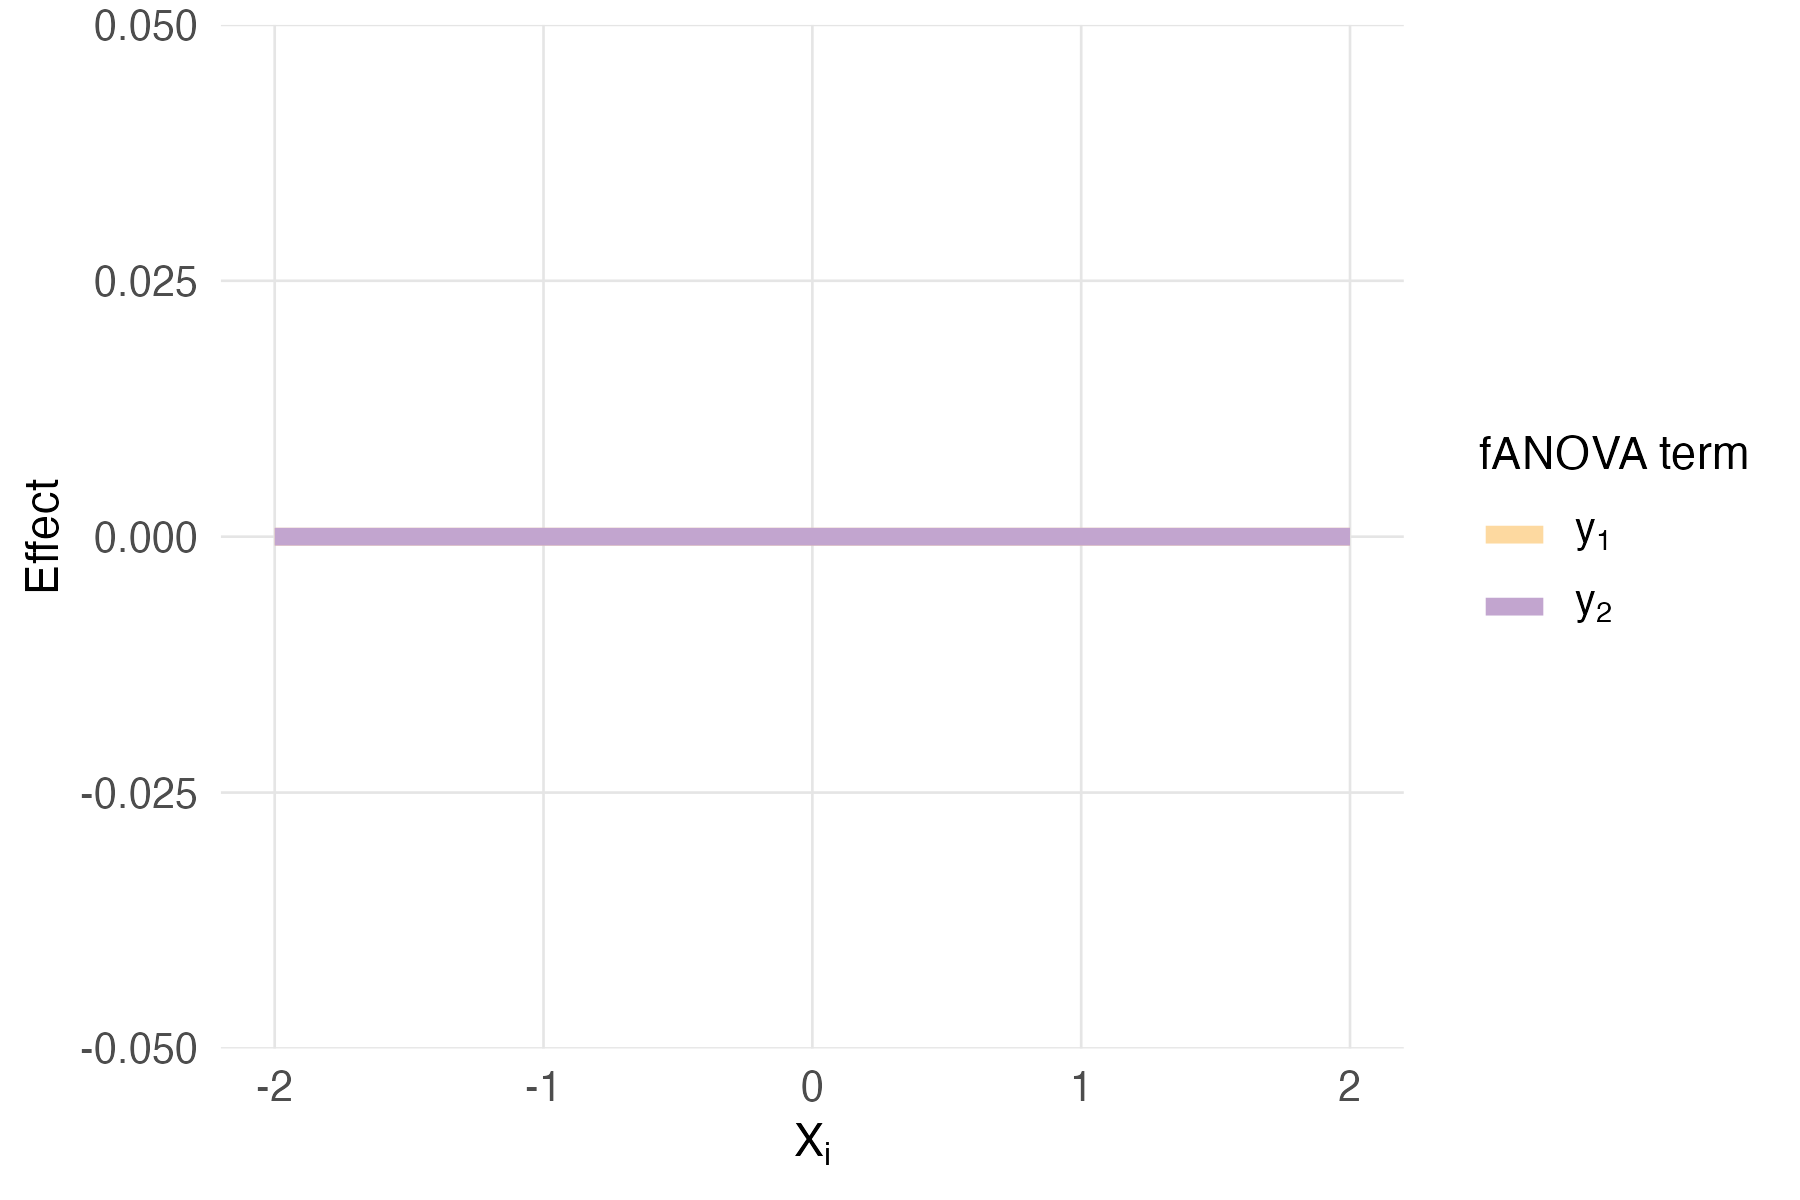
\includegraphics[width=\textwidth]{images/experiment_section/interaction_a1p00_a2p00_a11p00_a22p00_a12p20_rhop00_main.png}
        \caption{Main effects for $\rho = 0$}
    \end{subfigure}%
    \hfill
    \begin{subfigure}[t]{0.49\textwidth}
        \centering
        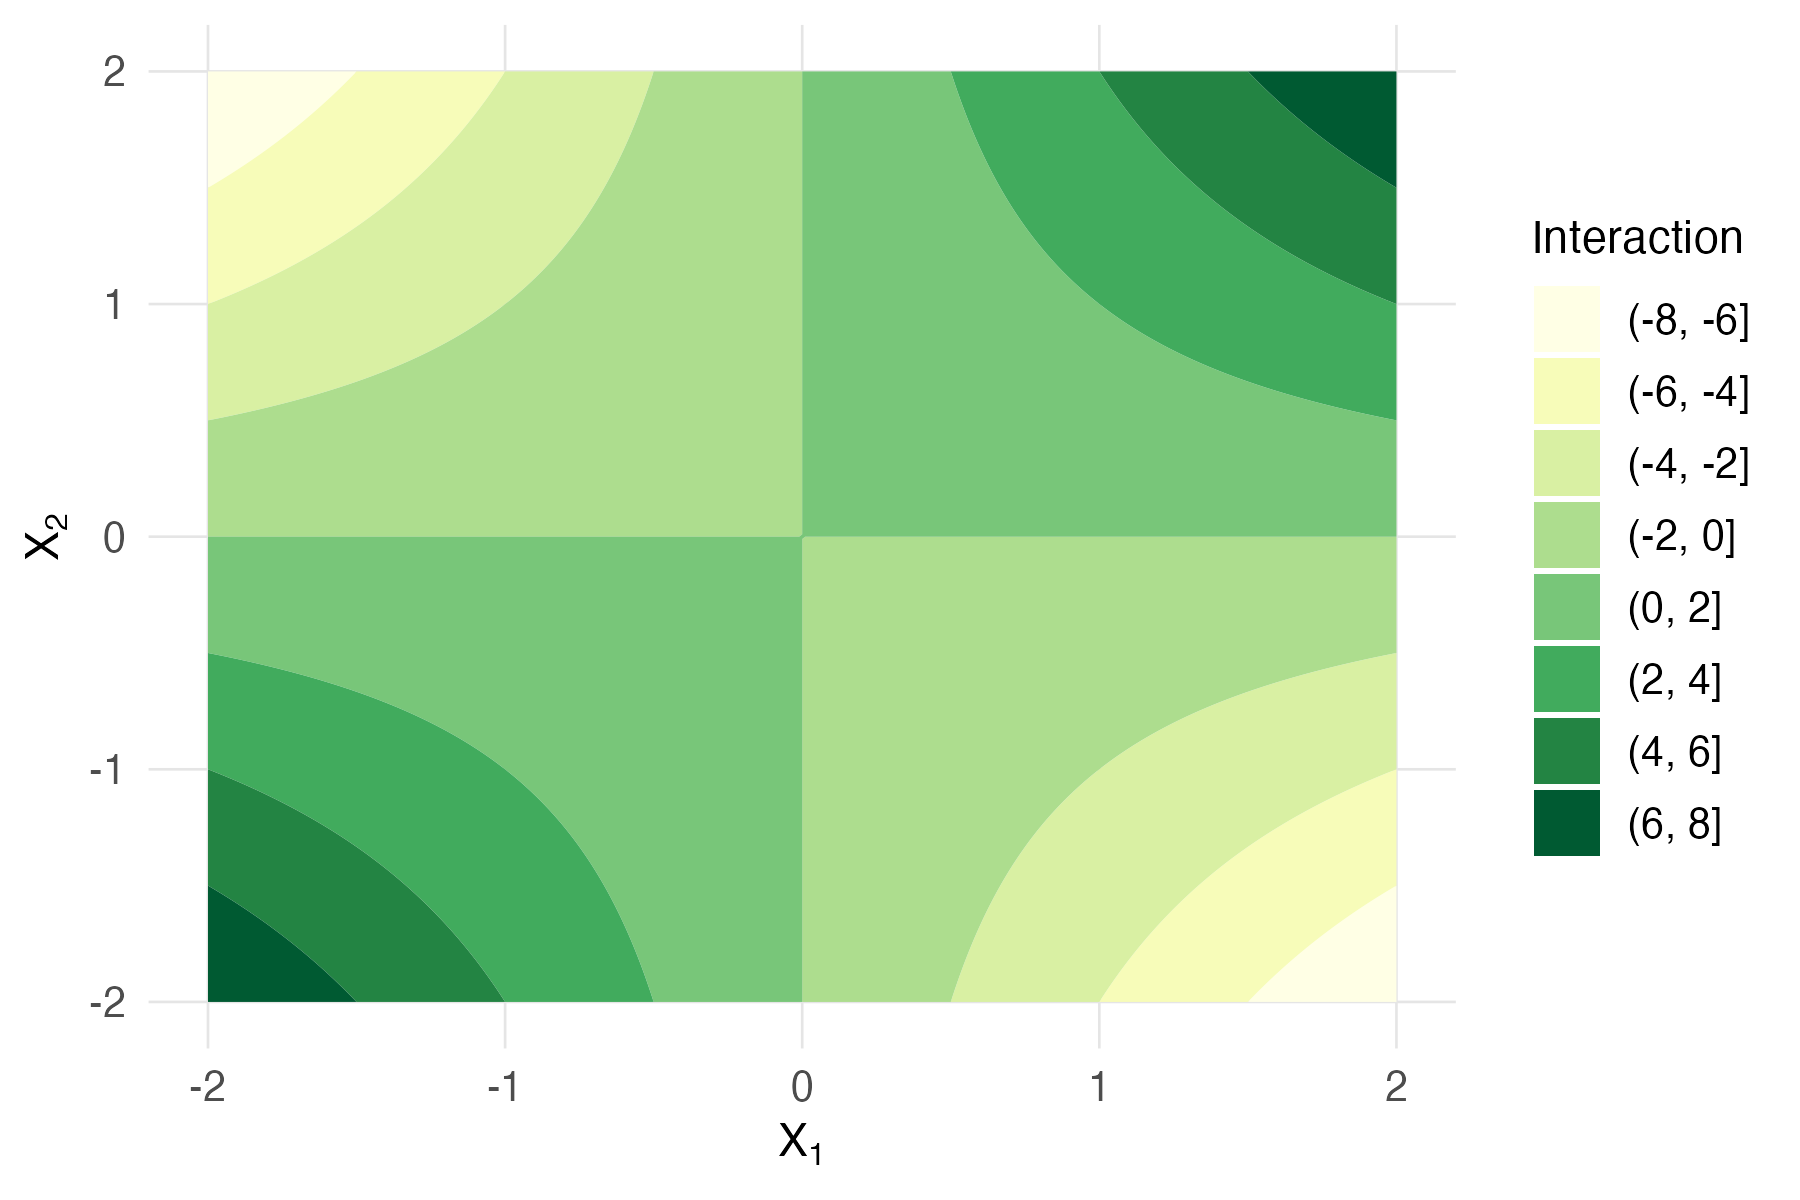
\includegraphics[width=\textwidth]{images/experiment_section/interaction_a1p00_a2p00_a11p00_a22p00_a12p20_rhop00_interaction.png}
        \caption{Interaction contour for $\rho = 0$}
    \end{subfigure}

    \vspace{0.5em}
    % ----- Row 3 -----
    \begin{subfigure}[t]{0.49\textwidth}
        \centering
        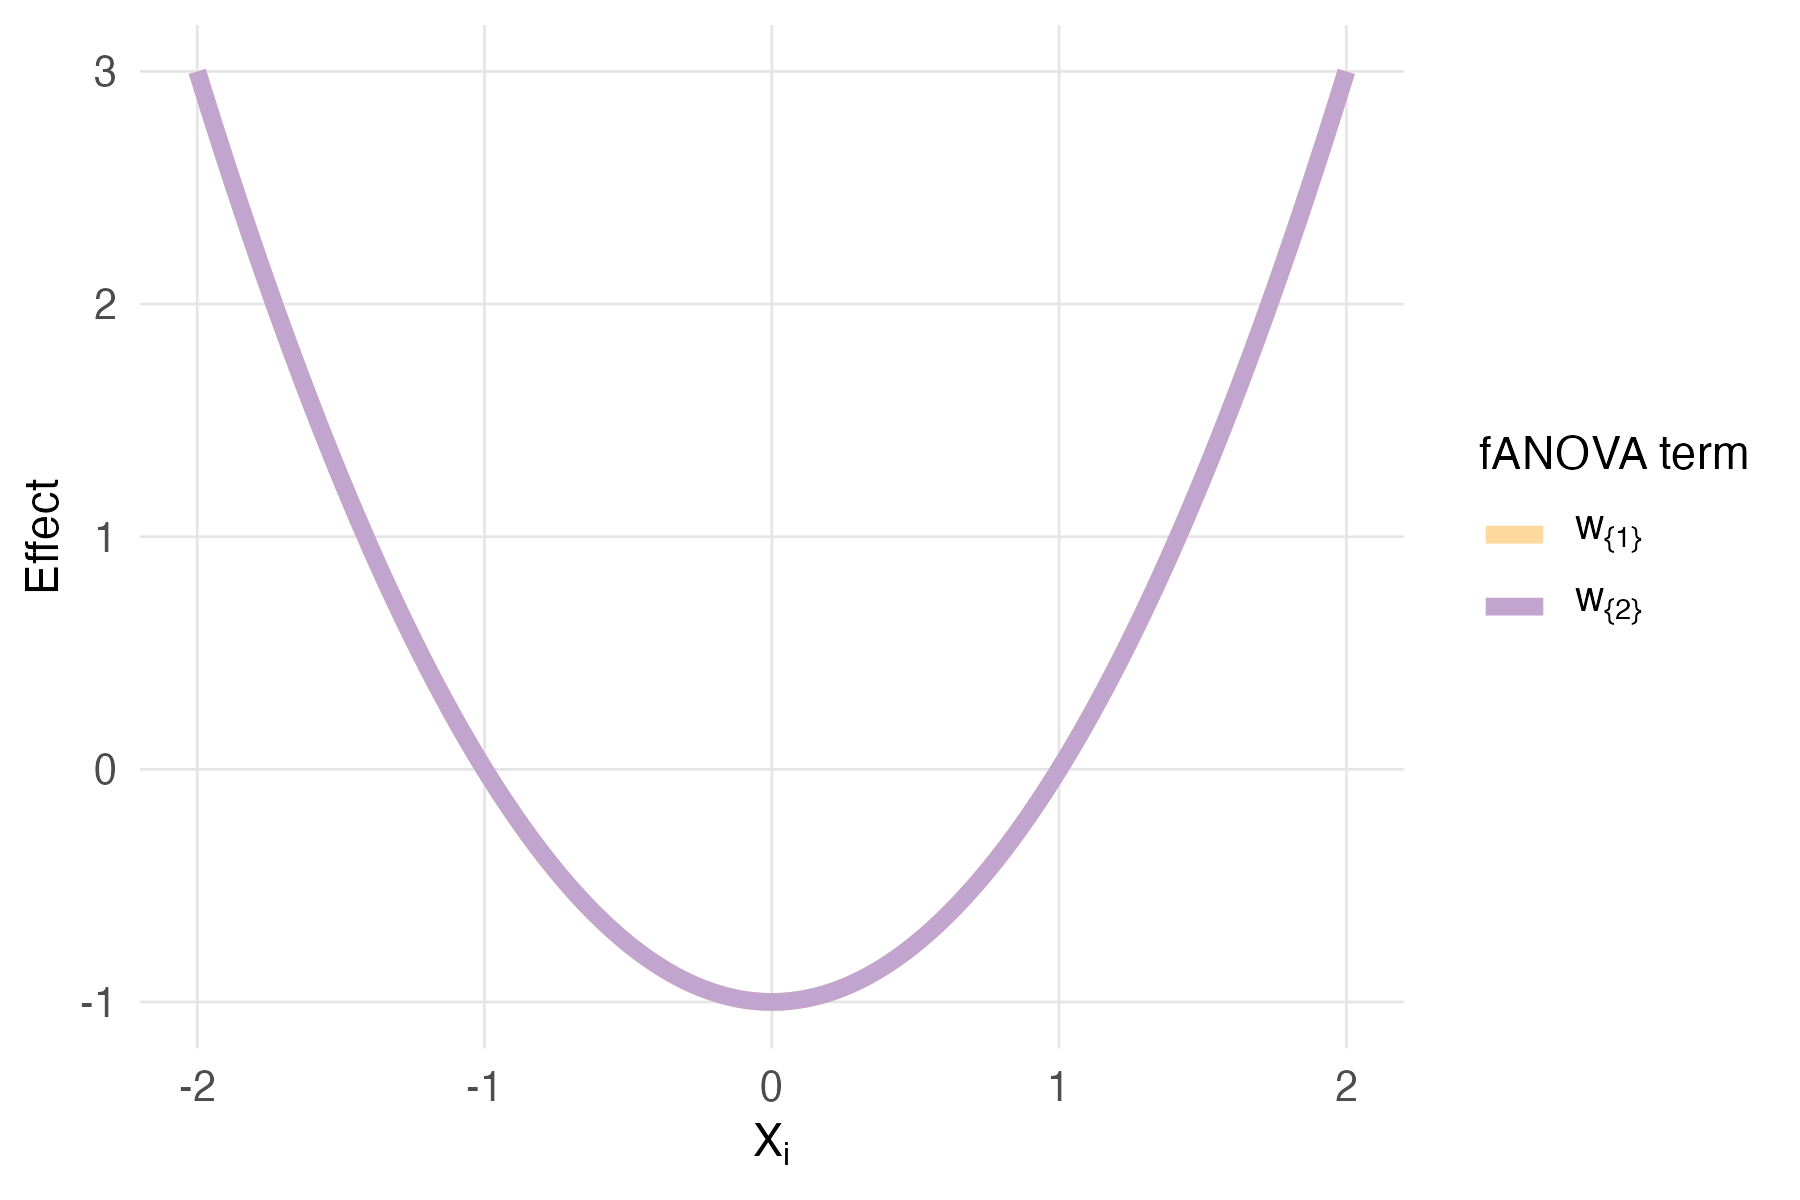
\includegraphics[width=\textwidth]{images/experiment_section/interaction_a1p00_a2p00_a11p00_a22p00_a12p20_rhop10_main.png}
        \caption{Main effects for $\rho = 1$}
    \end{subfigure}%
    \hfill
    \begin{subfigure}[t]{0.49\textwidth}
        \centering
        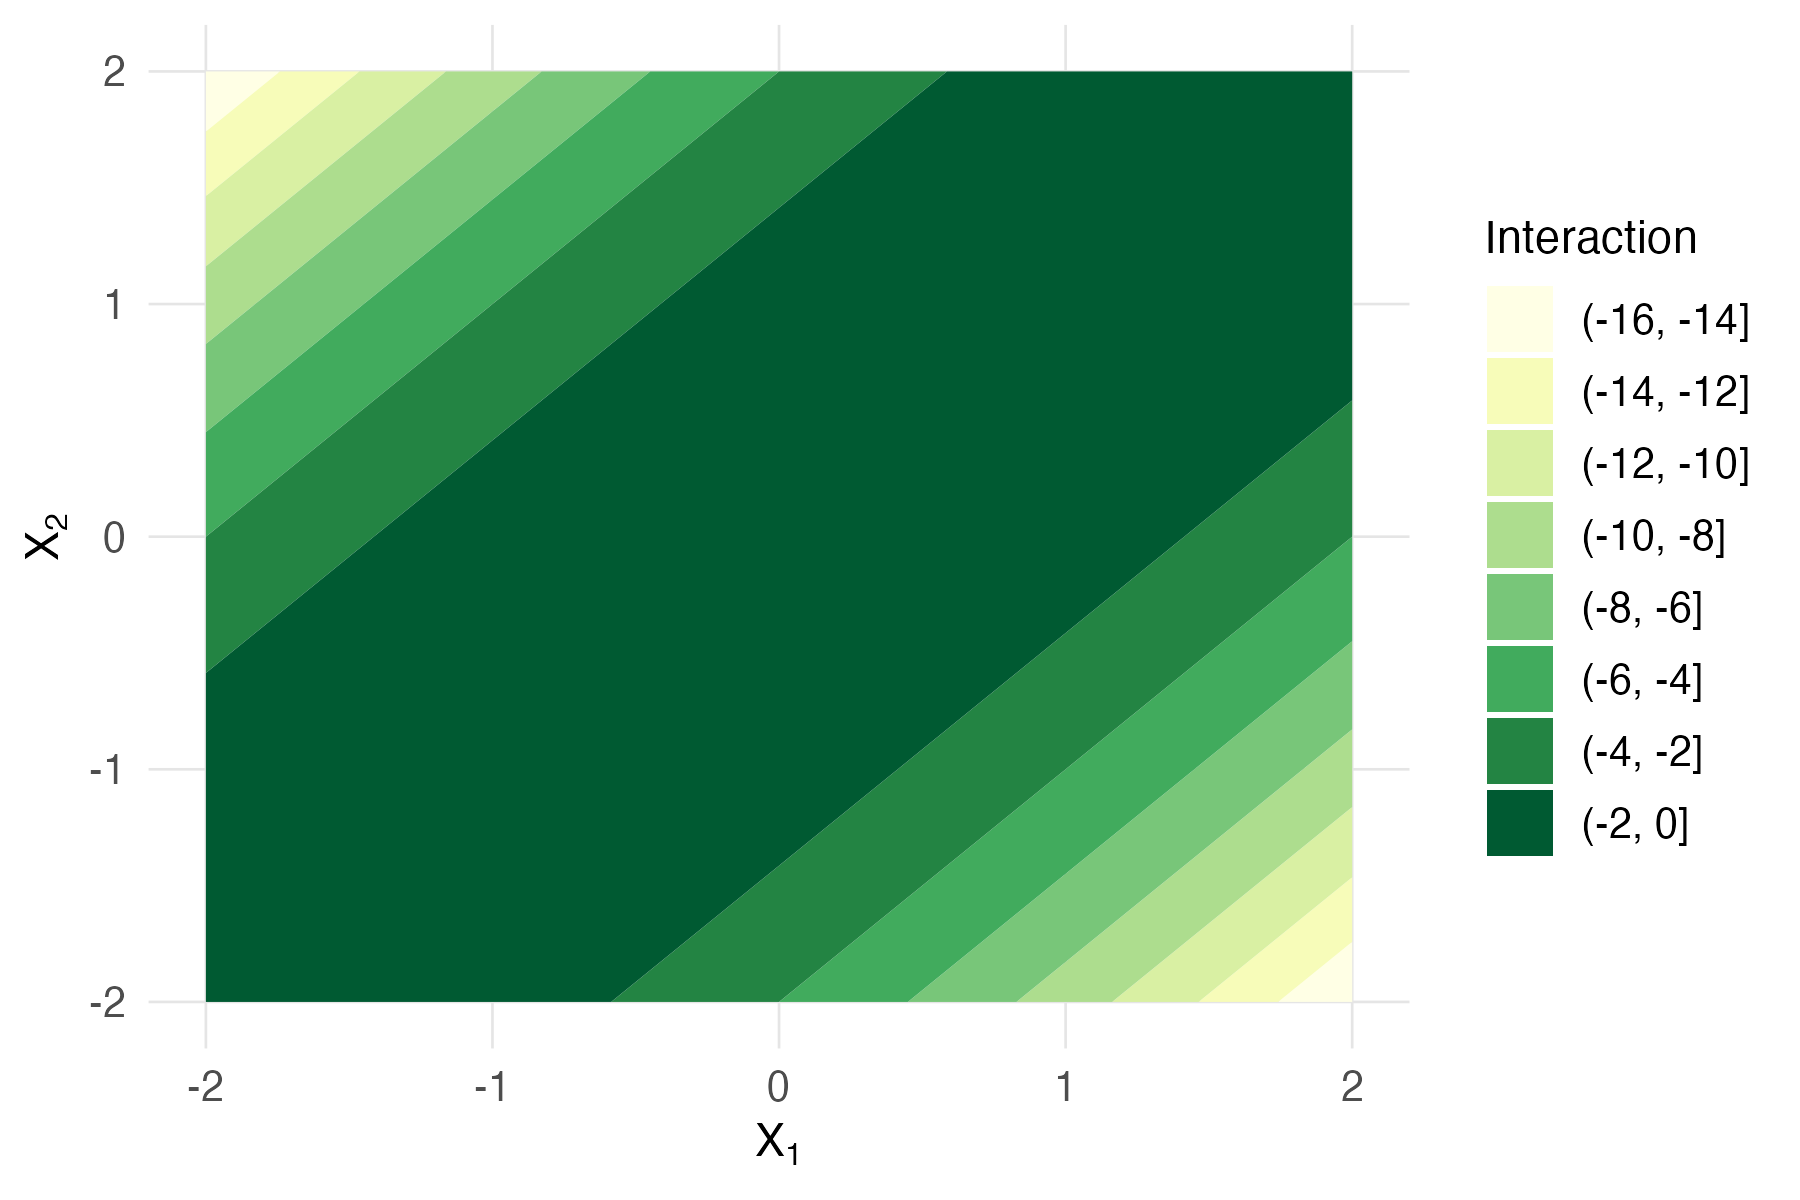
\includegraphics[width=\textwidth]{images/experiment_section/interaction_a1p00_a2p00_a11p00_a22p00_a12p20_rhop10_interaction.png}
        \caption{Interaction contour for $\rho = 1$}
    \end{subfigure}

    \caption{Main effects (left column) and interaction contour plots (right column) for different values of $\rho$. The effects are given by $y_{1}(x_1) = a_{12} \frac{\rho}{1+ \rho} (x_1^2 - 1)$,
    $y_{2}(x_2) = a_{12} \frac{\rho}{1+ \rho} (x_2^2 - 1)$,
    $y_{12}(x_1,x_2) = -a_{12}\!\left(\frac{\rho(x_1^2+x_2^2)}{1+\rho^2} - x_1 x_2 + \frac{\rho(\rho^2-1)}{1+\rho^2}\right)$.}
    \label{fig:interaction_combined}
\end{figure}

\subsubsection{Scenario: Full}
Finally, a full example, including all main and interaction effects:
$$g_4(x_1, x_2) = a_1 x_1 + a_2 x_2 + a_{11} x_1^2 + a_{22} x_2^2 + a_{12} x_1 x_2.$$
Now the fANOVA components are given by \autoref{eq:fanova_components_2D_polynomial}, where $a_0 = 0$.
We can vary the coefficients as well as $\rho$.\par
When the true function has no interaction term, as in our first two scenarios, varying $\rho$ is uninteresting because there is no way it could influence the form of the main effects. In this full scenario, however, there is an interaction term present, and therefore it is most interesting to compare pairs of coefficient sets under $\rho = 0$ versus $\rho \neq 0$. With this we want to essentially ask how effects are distorted by performing the classical fANOVA decomposition when a true interaction effect is present and variables exhibit dependency (or is this nonsense because we essentially did this with our running example?).
In \autoref{fig:all_pair_01} we make this comparison for a weak linear correlation between variables and in \autoref{fig:all_pair_02} we show the same for a strong linear correlation between variables. Similar to our running example at the beginning of this section, we see that main effects are distorted slightly, while interaction effects look substantially different under dependent inputs.

\begin{figure}[htpb]
    \centering

    % -------- Pair 1.1 --------
    \begin{subfigure}[t]{\textwidth}
        \centering
        \begin{minipage}[t]{0.49\textwidth}
            \centering
            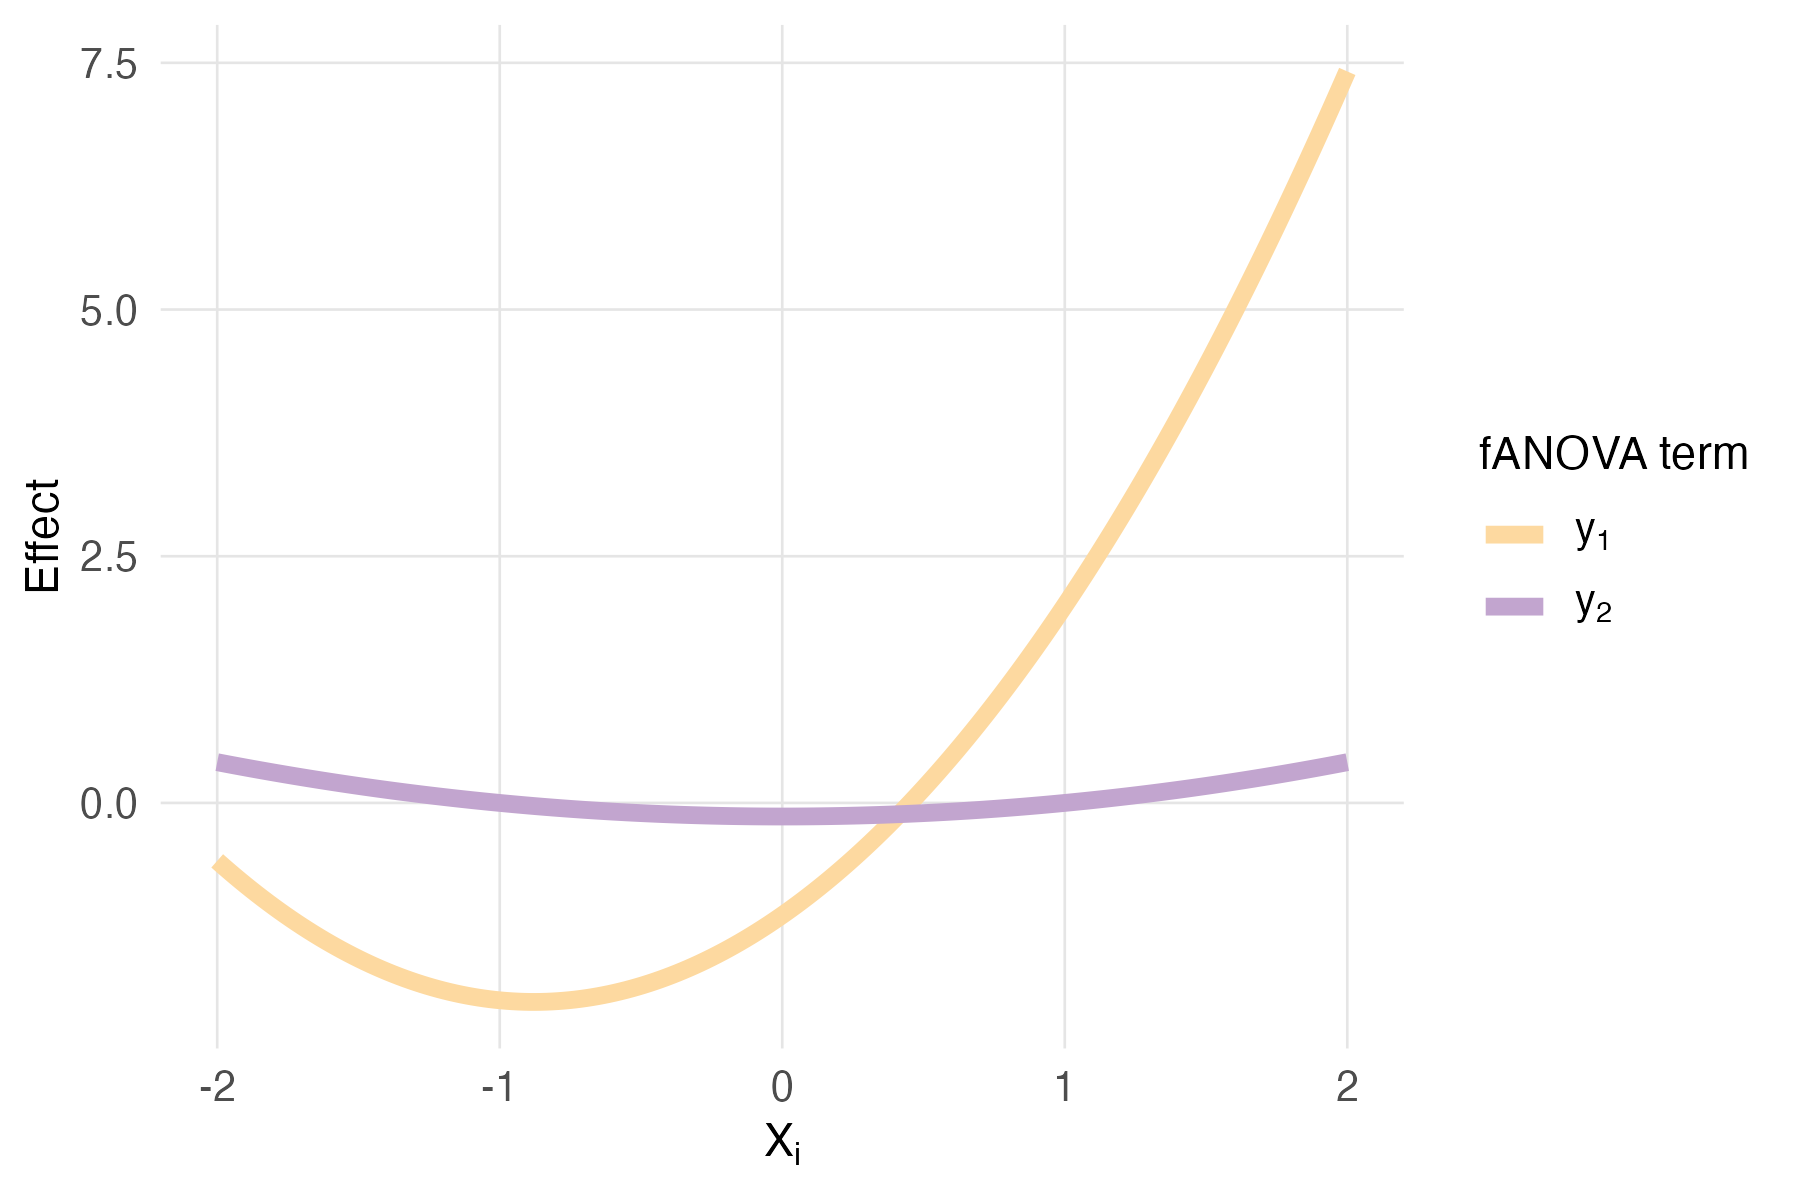
\includegraphics[width=\textwidth]{images/experiment_section/full_a1p20_a2p00_a11p10_a22p00_a12p05_rhop03_main.png}
        \end{minipage}%
        \hfill
        \begin{minipage}[t]{0.49\textwidth}
            \centering
            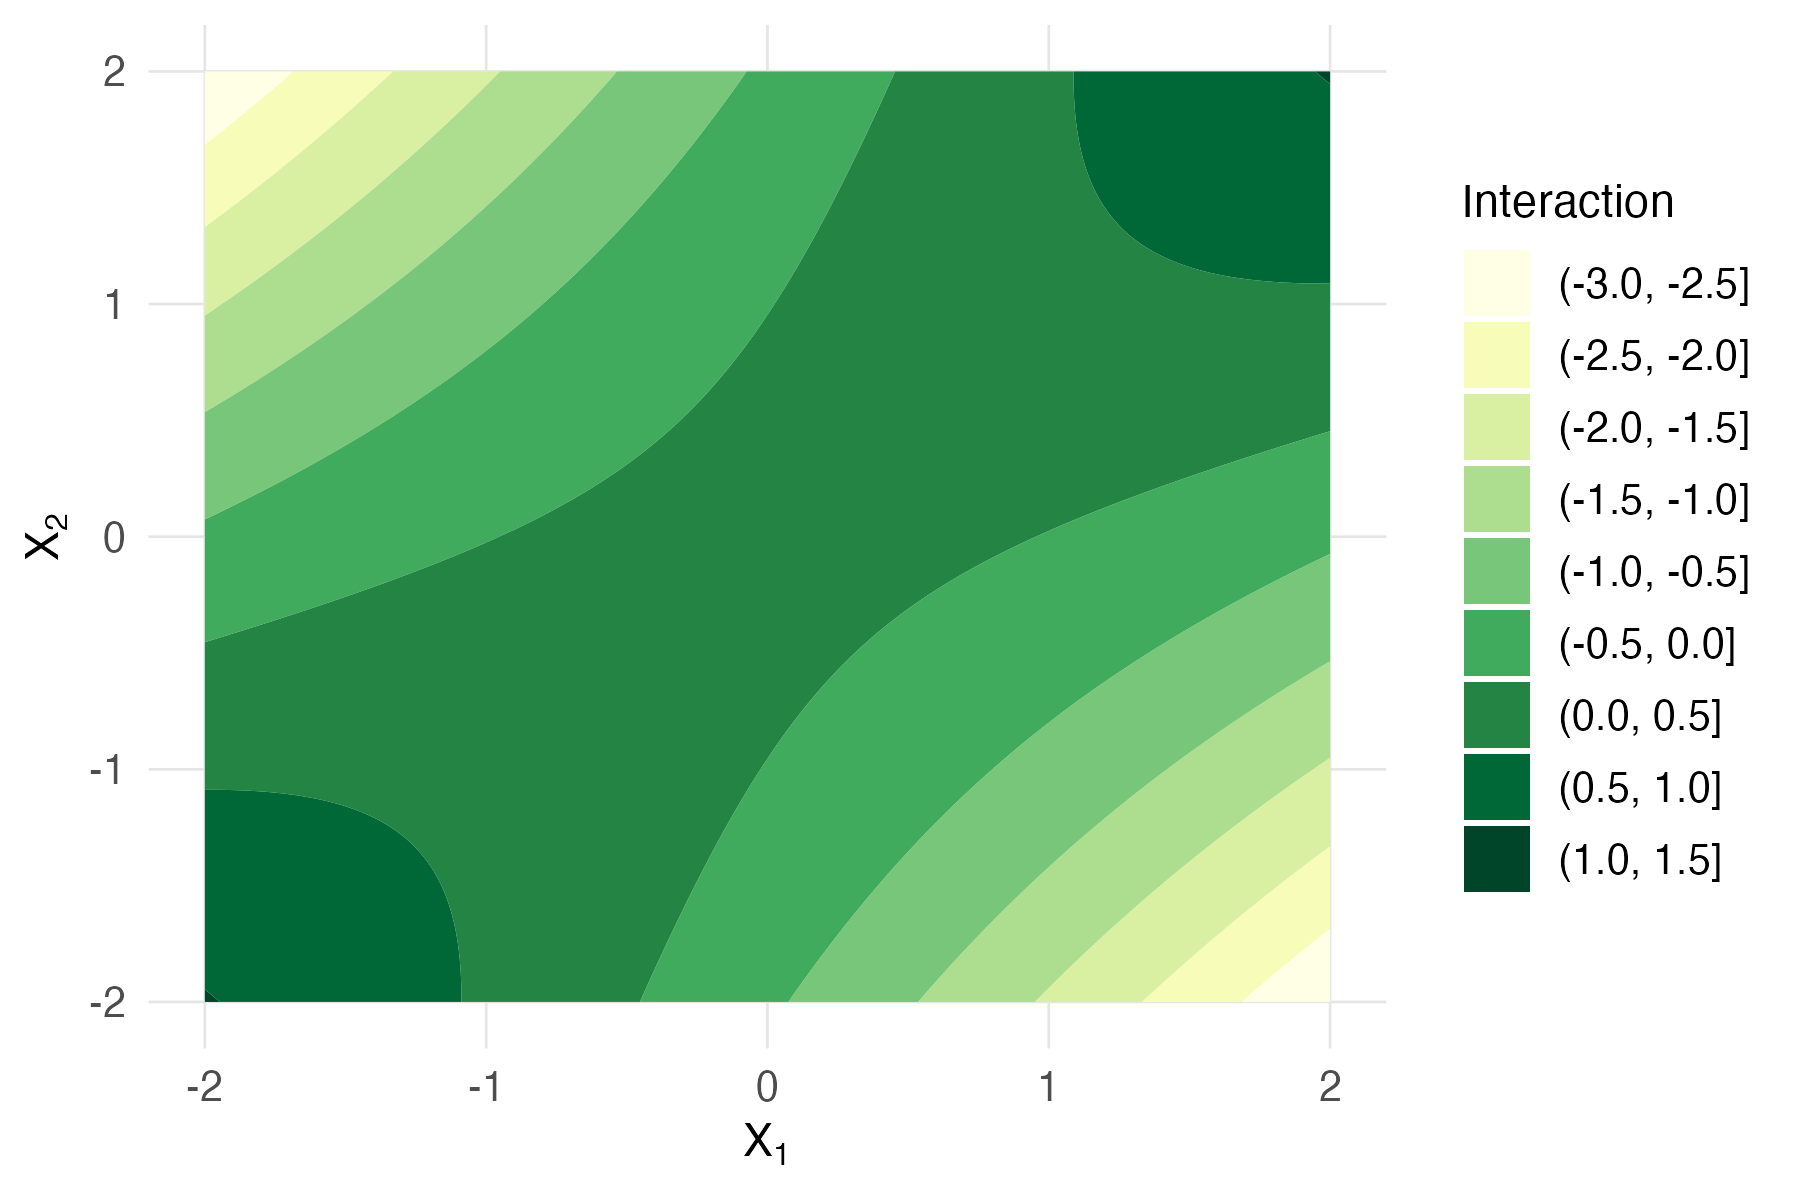
\includegraphics[width=\textwidth]{images/experiment_section/full_a1p20_a2p00_a11p10_a22p00_a12p05_rhop03_interaction.png}
        \end{minipage}
        \caption{Main and interaction effects for (1) $a_1 = 2$, $a_2 = 0$, 
                 $a_{11} = 1$, $a_{22} = 0$, $a_{12} = 0.5$, $\rho = 0.3$.}
    \end{subfigure}

    % -------- Pair 1.2 --------
    \begin{subfigure}[t]{\textwidth}
        \centering
        \begin{minipage}[t]{0.49\textwidth}
            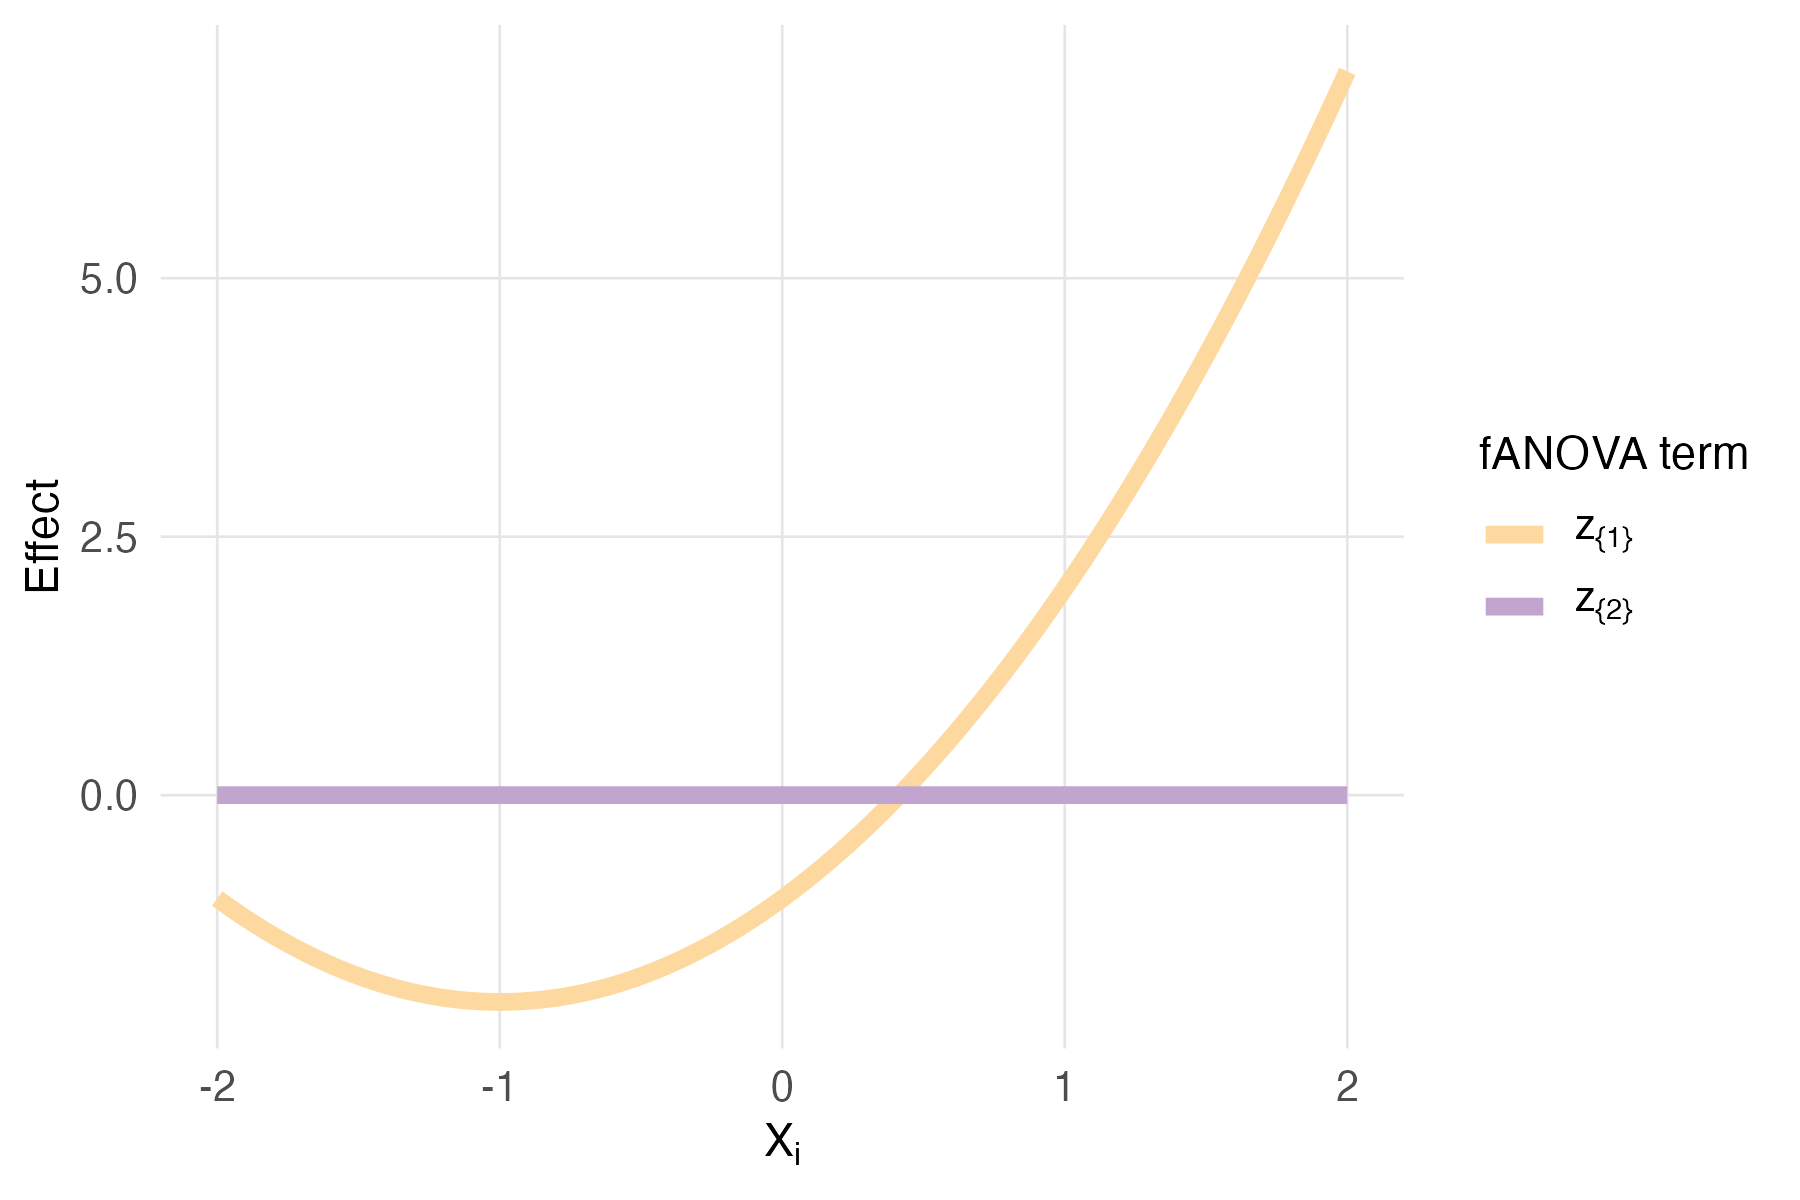
\includegraphics[width=\textwidth]{images/experiment_section/full_a1p20_a2p00_a11p10_a22p00_a12p05_rhop00_main.png}
        \end{minipage}%
        \hfill
        \begin{minipage}[t]{0.49\textwidth}
            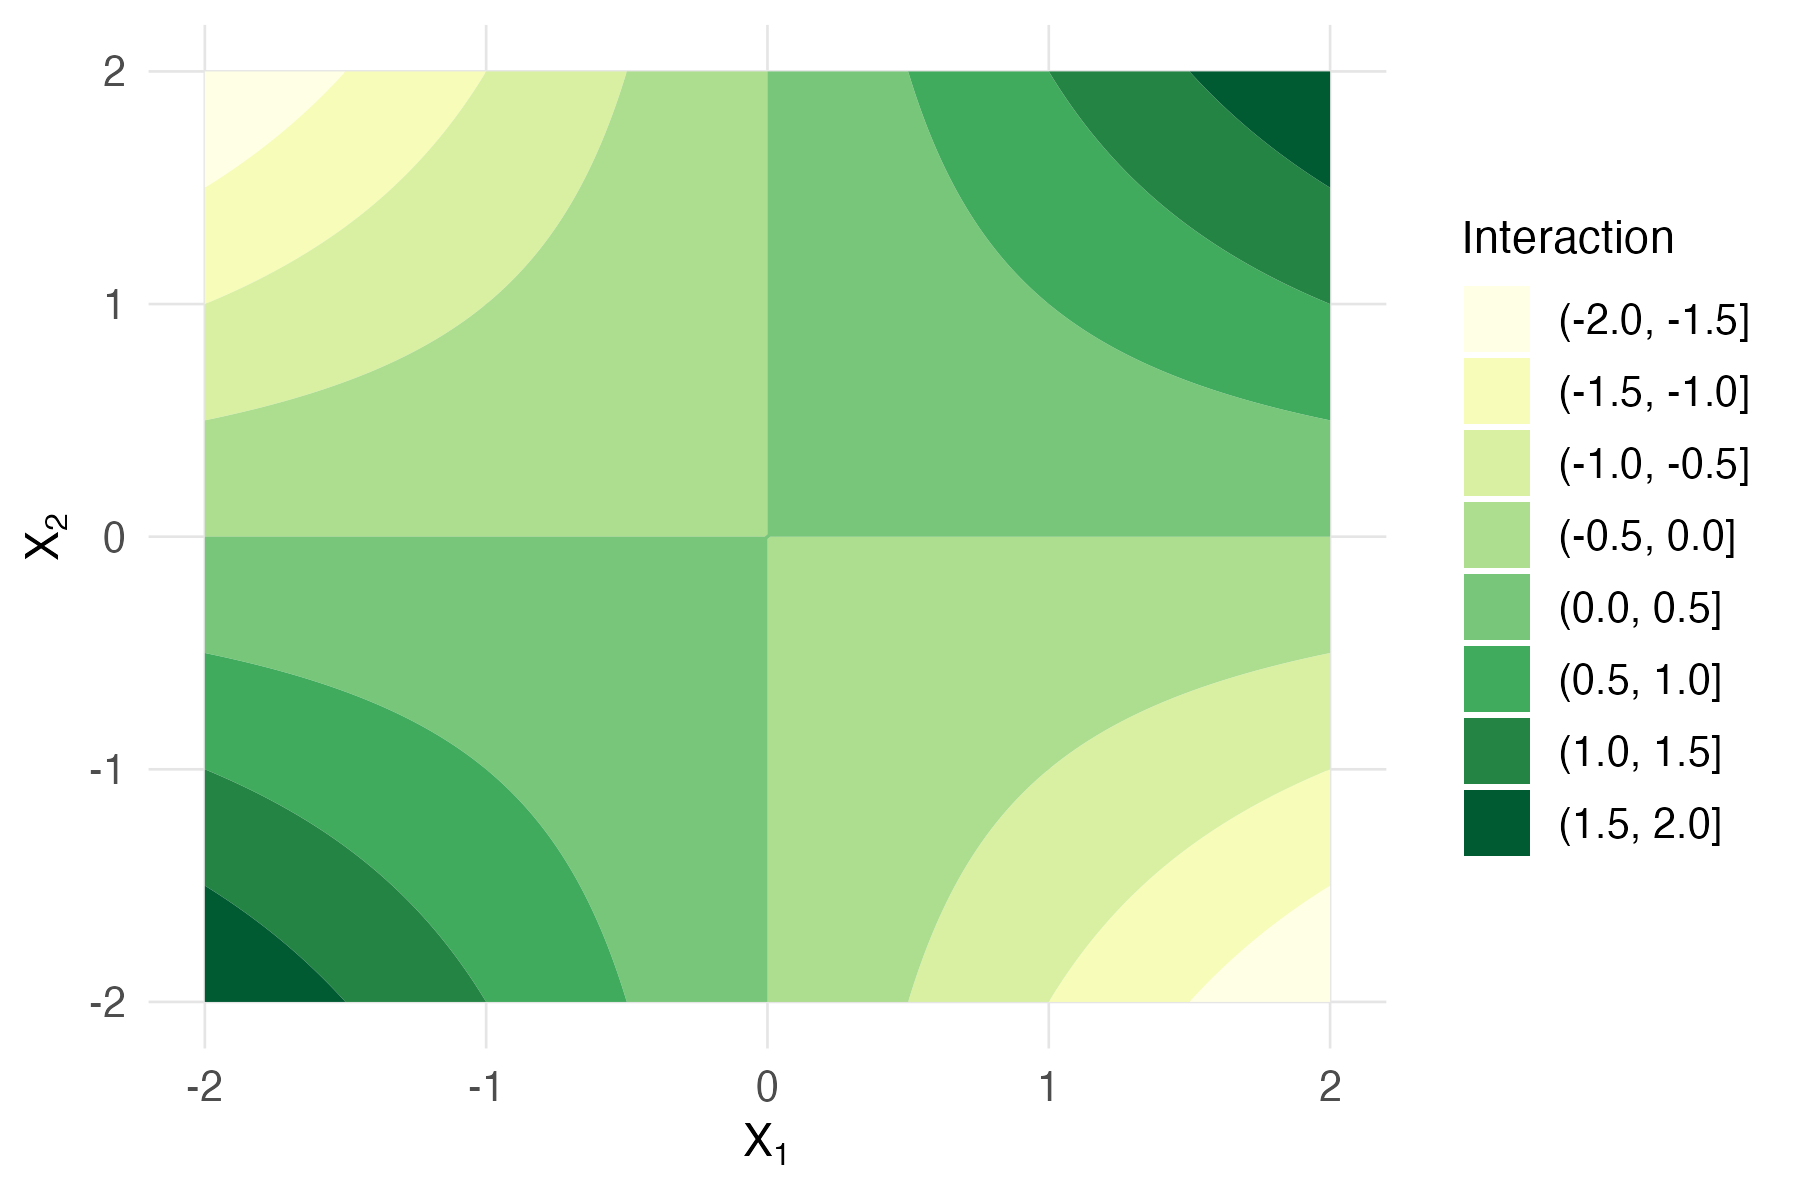
\includegraphics[width=\textwidth]{images/experiment_section/full_a1p20_a2p00_a11p10_a22p00_a12p05_rhop00_interaction.png}
        \end{minipage}
        \caption{Main and interaction effects for (2) $a_1 = 0$, $a_2 = 2$, 
                 $a_{11} = 0$, $a_{22} = 1$, $a_{12} = -0.5$, $\rho = 0$.}
    \end{subfigure}
    \caption{Main effects (left) and interaction contours (right) for four different coefficient sets.}
    \label{fig:all_pair_01}
\end{figure}

\begin{figure}[htpb]
    \centering
    % -------- Pair 2.1 --------
    \begin{subfigure}[t]{\textwidth}
        \centering
        \begin{minipage}[t]{0.49\textwidth}
            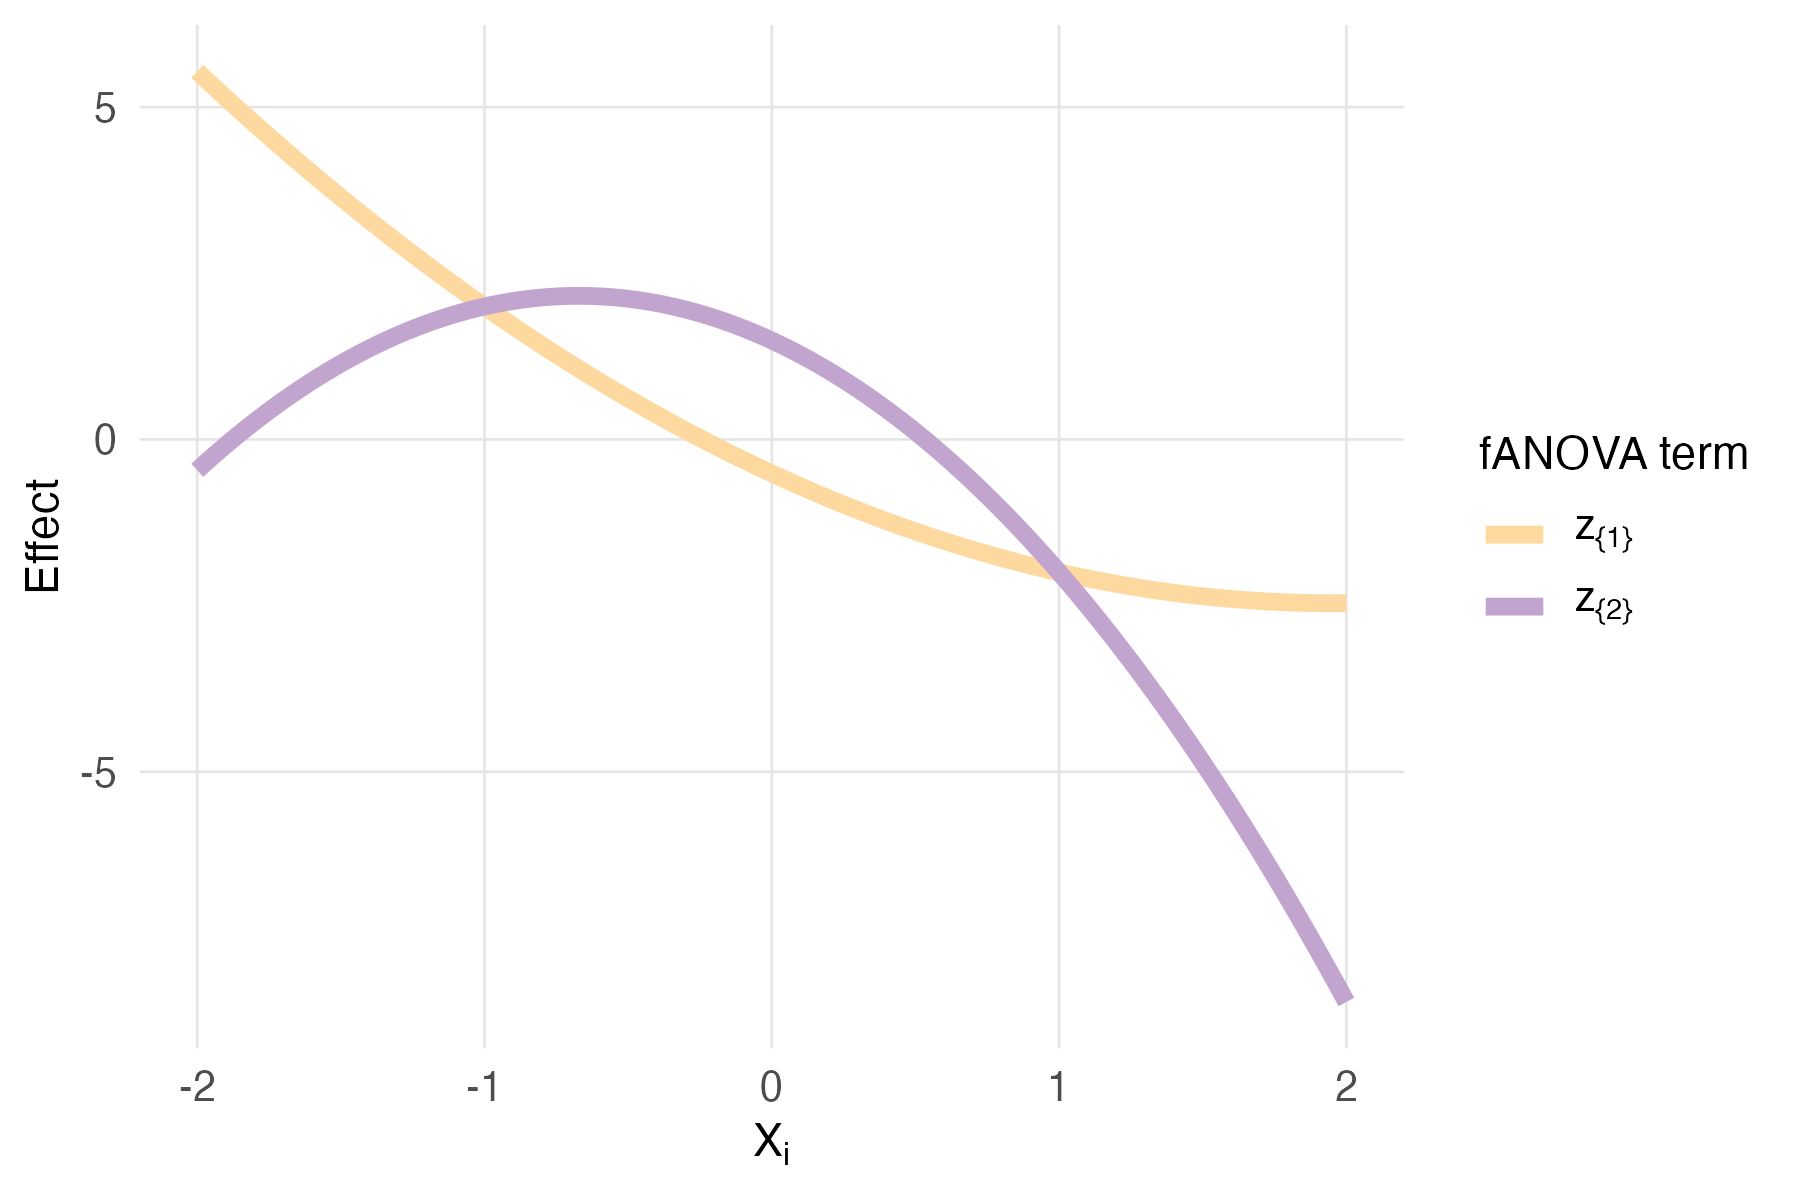
\includegraphics[width=\textwidth]{images/experiment_section/full_a1m20_a2m20_a11p10_a22m10_a12p10_rhom08_main.png}
        \end{minipage}%
        \hfill
        \begin{minipage}[t]{0.49\textwidth}
            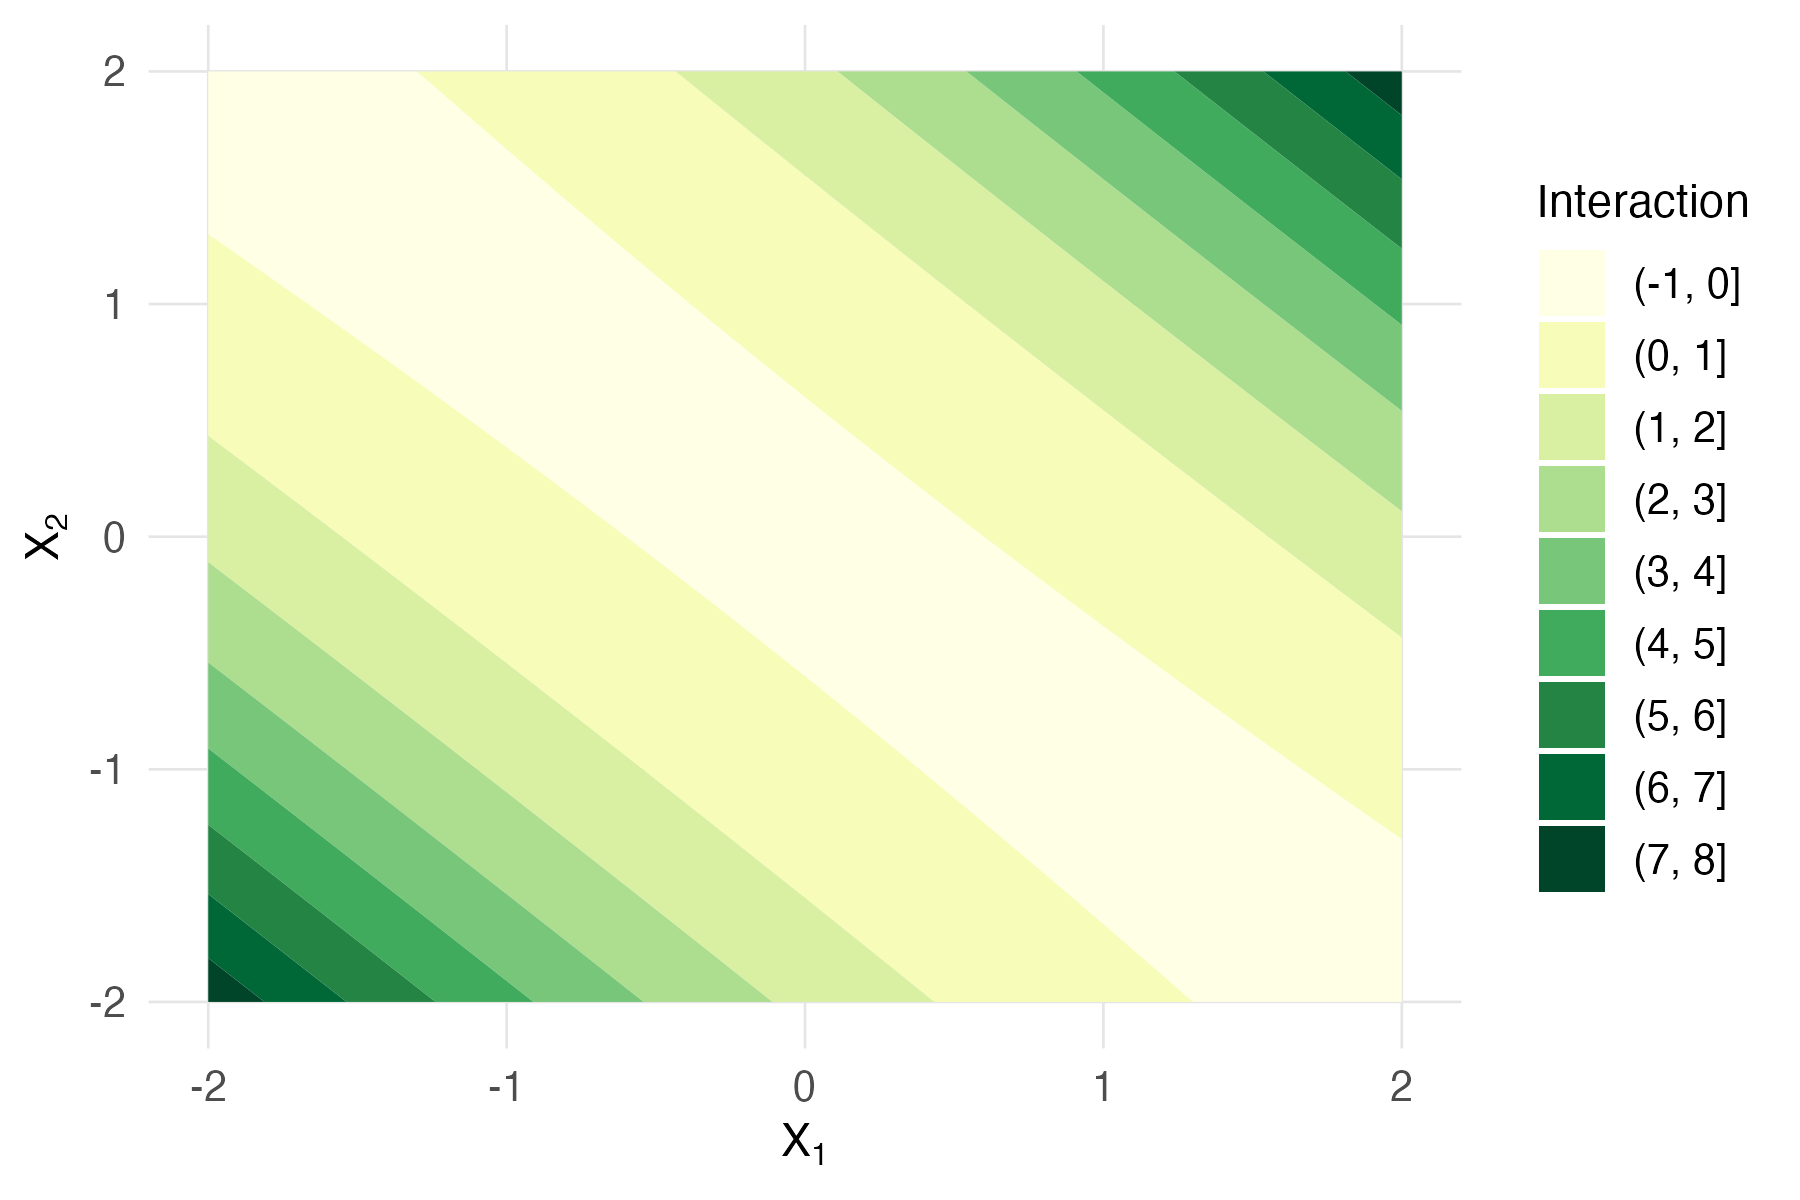
\includegraphics[width=\textwidth]{images/experiment_section/full_a1m20_a2m20_a11p10_a22m10_a12p10_rhom08_interaction.png}
        \end{minipage}
        \caption{Main and interaction effects for (3) $a_1 = -2$, $a_2 = -2$, 
                 $a_{11} = 1$, $a_{22} = -1$, $a_{12} = 1$, $\rho = -0.8$.}
    \end{subfigure}

    % -------- Pair 2.2 --------
    \begin{subfigure}[t]{\textwidth}
        \centering
        \begin{minipage}[t]{0.49\textwidth}
            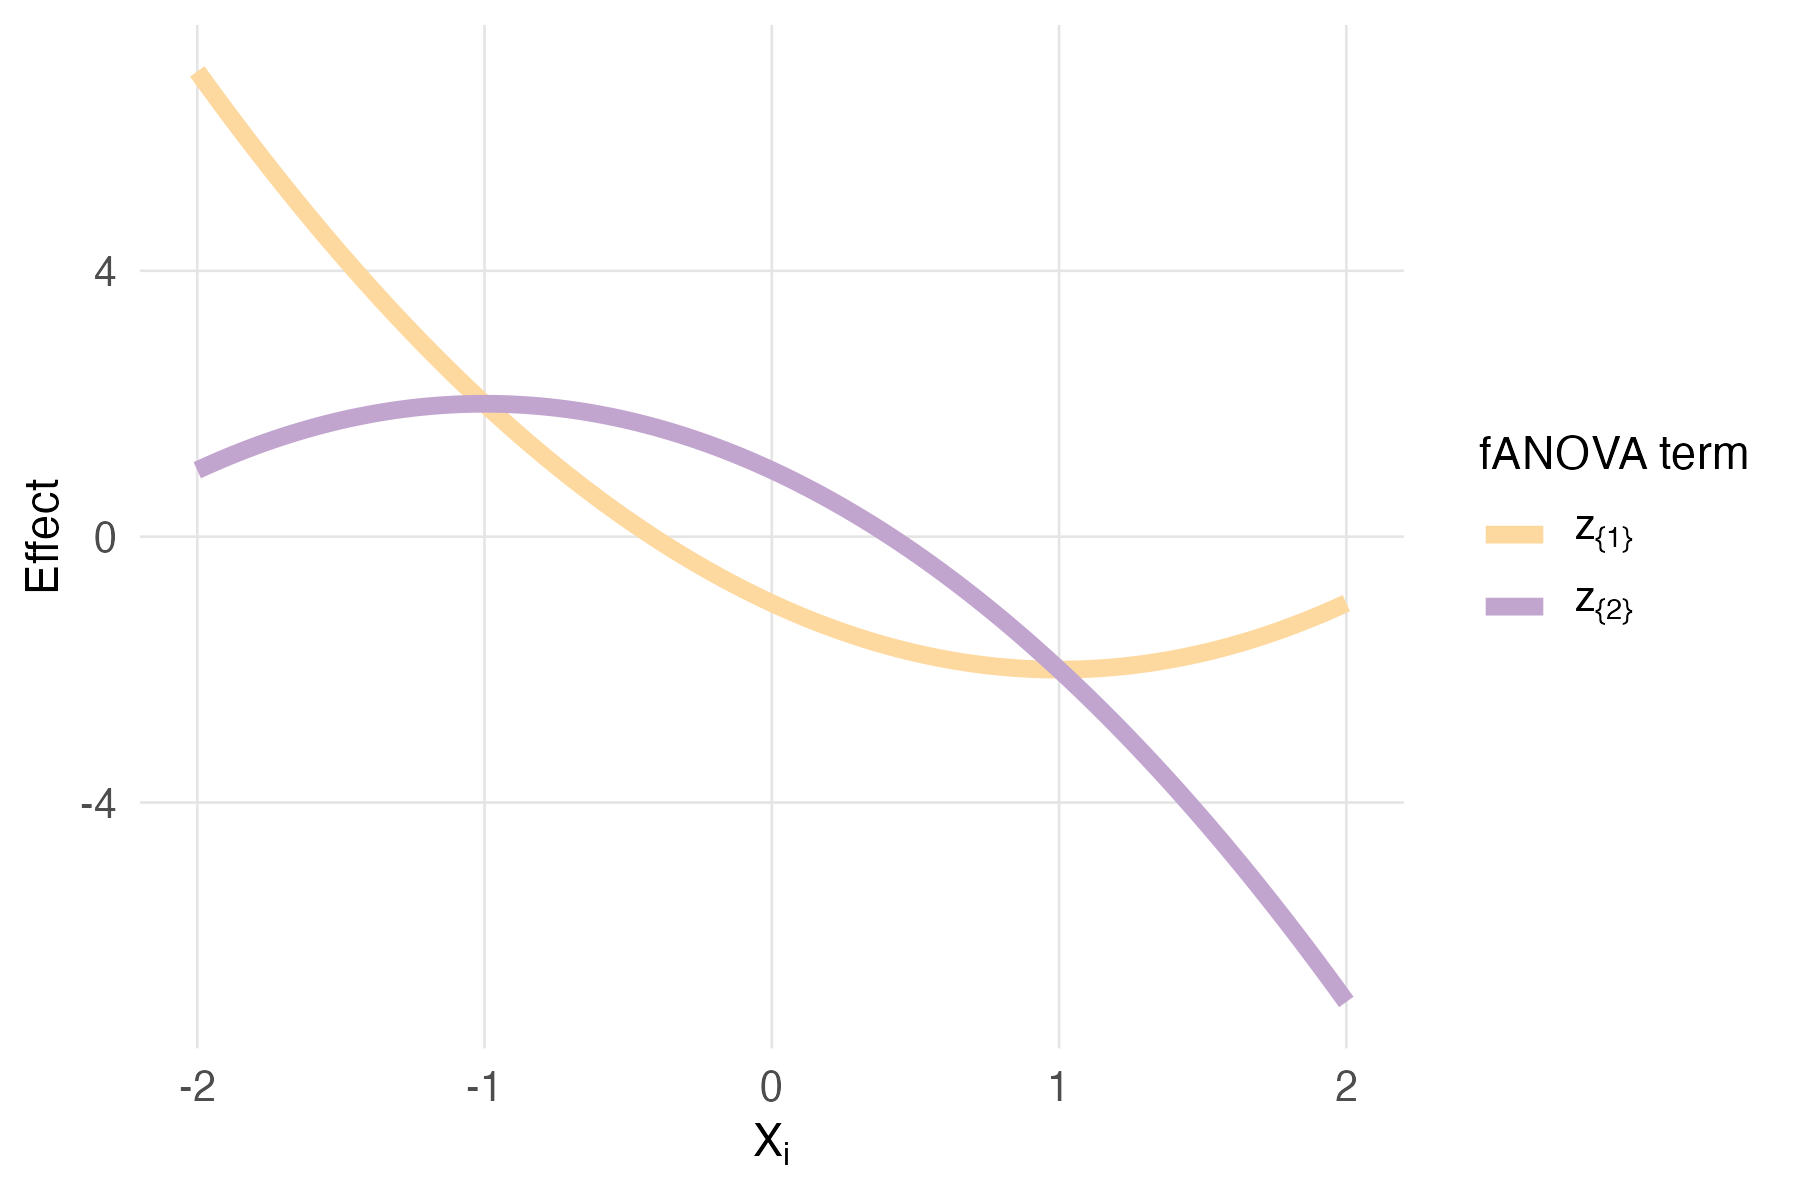
\includegraphics[width=\textwidth]{images/experiment_section/full_a1m20_a2m20_a11p10_a22m10_a12p10_rhop00_main.png}
        \end{minipage}%
        \hfill
        \begin{minipage}[t]{0.49\textwidth}
            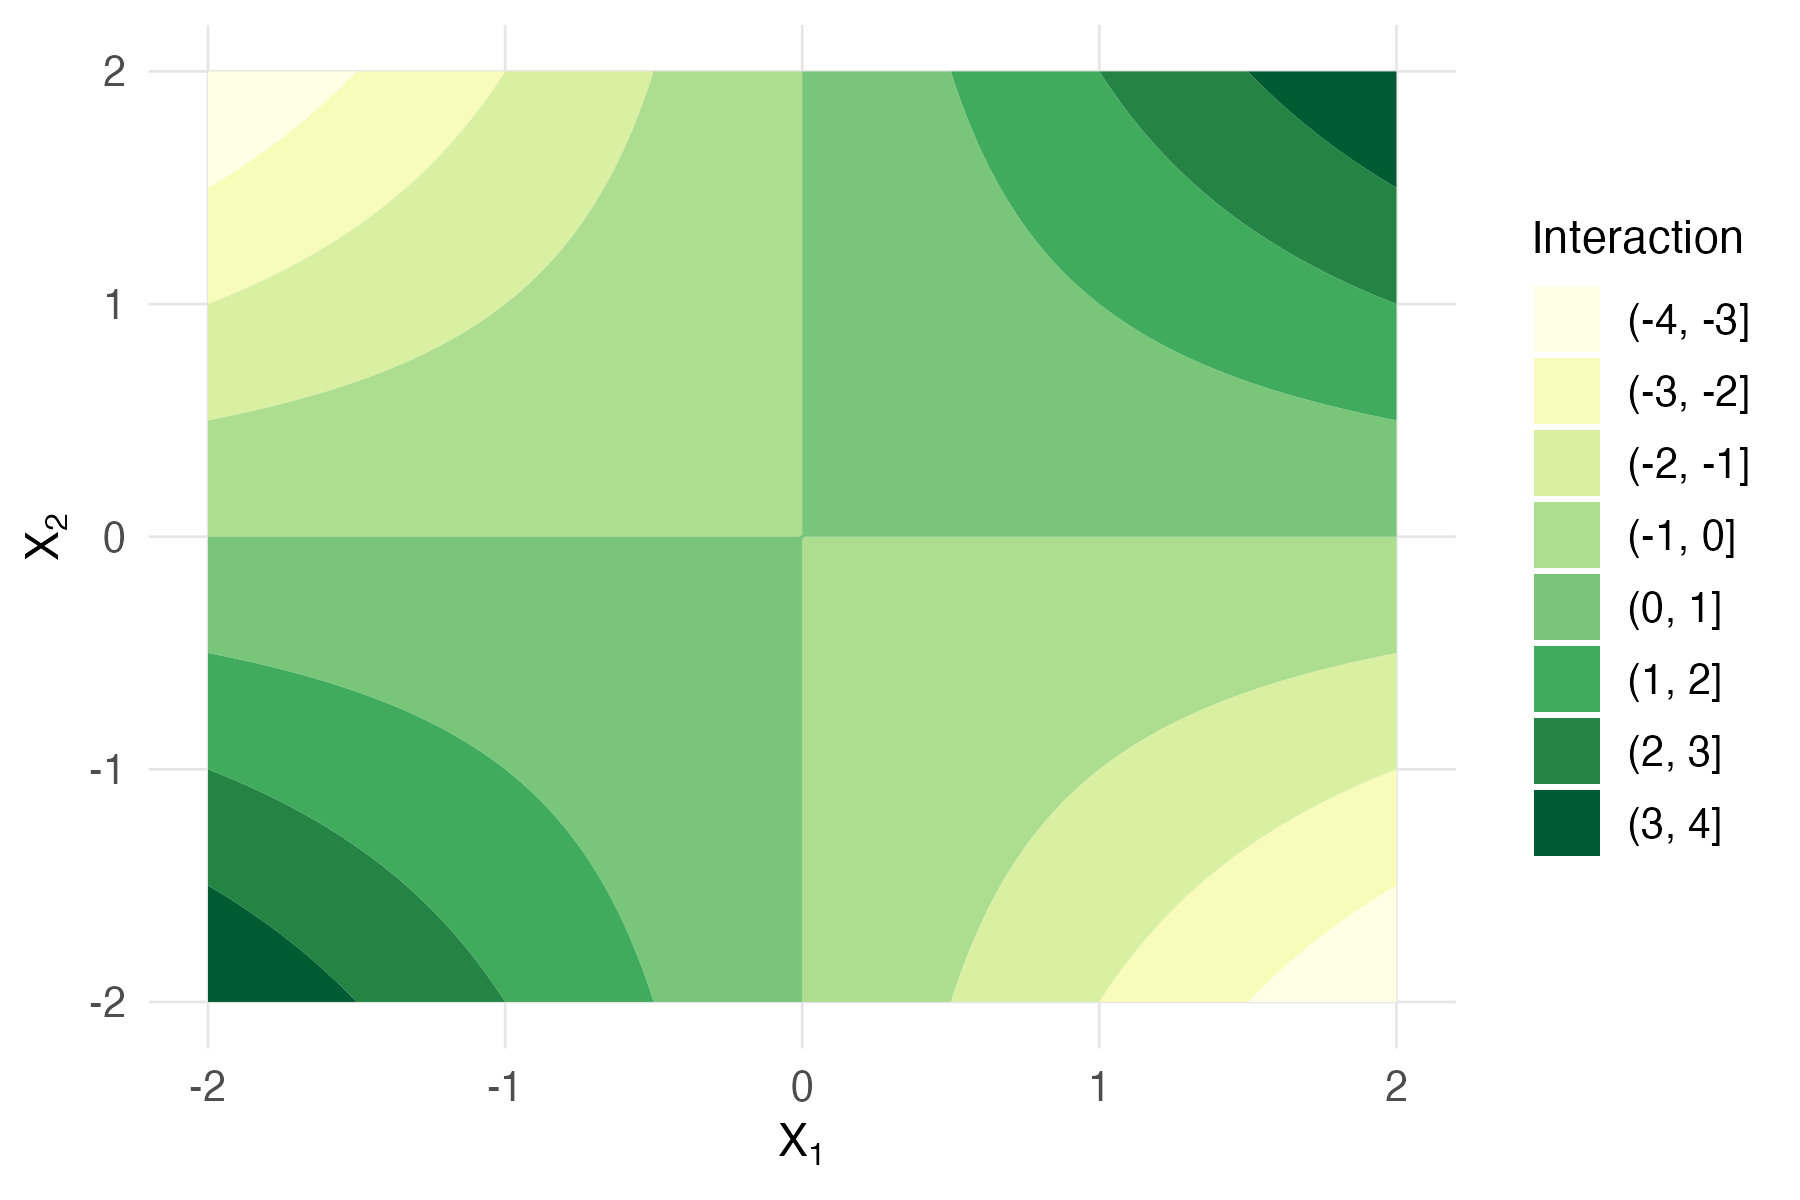
\includegraphics[width=\textwidth]{images/experiment_section/full_a1m20_a2m20_a11p10_a22m10_a12p10_rhop00_interaction.png}
        \end{minipage}
        \caption{Main and interaction effects for (4) $a_1 = -2$, $a_2 = 2$, 
                 $a_{11} = -1$, $a_{22} = 1$, $a_{12} = -1$, $\rho = 0$.}
    \end{subfigure}

    \caption{Main effects (left) and interaction contours (right) for four different \\ coefficient sets.}
    \label{fig:all_pair_02}
\end{figure}

\subsection{Estimation of fANOVA components}
This was all pretty theoretical and the examples we used foster understanding, but they are toy examples and in reality the true function is unknown and more complex. So to become a more widely used, established interpretability method, an estimation scheme is inevitable.
% Here we briefly present two estimation approaches by \cite{hooker2004, hooker2007},
We already encountered one estimation scheme proposed by \cite{rahman2014} when computing the generalized fANOVA components for our running example; we refer to \autoref{sec:formalization_fANOVA} the conceptual idea behind it.

In \cite{hooker2004} an estimation framework based on partial dependence is proposed, which makes use of the formulation of fANOVA via projections. To obtain the component estimate for $y_u$, Hooker proposed to estimate the projections of $y$ onto the subspace of variables spanned by $u$ empirically.
One does so by first estimating the conditional expected value of the variables in $u$. % (keep variables in $u$ fixed an average over all others).
This is a simple Monte Carlo estimation, which results in the partial dependence function (PD Function) for the variables in $u$ \citep{hooker2004}.
The PD Function can then be used to estimate the empirical projection of interest. He states that his method works well for functions that have nearly additive true structure and purely additive functions are exactly recoverable with this approach. However, the approach suffers from extrapolation issues or artefacts when the true function involves interactions and inputs are dependent.\par


Therefore, in \cite{hooker2007} a new estimation scheme is proposed for his version of the generalized fANOVA decomposition (see \autoref{sec:formalization_fANOVA}).
Hooker rewrites his proposed system of equations as restricted weighted least squares problem and solves it via Lagrange multiplier for the exact solution of the simultaneously defined generalized components.
The function is evaluated at a grid of points to reduce computational costs.
Because of the parallel to weighted least squares, it is also possible to compute a weighted standard ANOVA with existing software; however, like so it is difficult to incorporate the system constraints and one might obtain components that are not hierarchical orthogonal.\par

None of these estimation approaches has a standard software implementation or published code.
Some existing unfinished implementations are numerically instable or yield illogical results. This underpins the need for a more robust estimation scheme with stable software implementation.
